\chapter{Universality and uncomputability}\label{chapcomputable}

\begin{objectives} \label[objectives]{The-universal-machineprog}

\begin{itemize}
\tightlist
\item
  The universal machine/program - ``one program to rule them all''
\item
  A fundamental result in computer science and mathematics: the
  existence of uncomputable functions.
\item
  The \emph{halting problem}: the canonical example of an uncomputable
  function.
\item
  Introduction to the technique of \emph{reductions}.
\item
  Rice's Theorem: A ``meta tool'' for uncomputability results, and a
  starting point for much of the research on compilers, programming
  languages, and software verification.
\end{itemize}

\end{objectives}

\begin{quote}
\emph{``A function of a variable quantity is an analytic expression
composed in any way whatsoever of the variable quantity and numbers or
constant quantities.''}, Leonhard Euler, 1748.
\end{quote}

\begin{quote}
\emph{``The importance of the universal machine is clear. We do not need
to have an infinity of different machines doing different jobs. \ldots{}
The engineering problem of producing various machines for various jobs
is replaced by the office work of `programming' the universal
machine''}, Alan Turing, 1948
\end{quote}

One of the most significant results we showed for Boolean circuits (or
equivalently, straight-line programs) is the notion of
\emph{universality}: there is a single circuit that can evaluate all
other circuits. However, this result came with a significant caveat. To
evaluate a circuit of \(s\) gates, the universal circuit needed to use a
number of gates \emph{larger} than \(s\). It turns out that uniform
models such as Turing machines or NAND-TM programs allow us to ``break
out of this cycle'' and obtain a truly \emph{universal Turing machine}
\(U\) that can evaluate all other machines, including machines that are
more complex (e.g., more states) than \(U\) itself. (Similarly, there is
a \emph{Universal NAND-TM program} \(U'\) that can evaluate all NAND-TM
programs, including programs that have more lines than \(U'\).)

It is no exaggeration to say that the existence of such a universal
program/machine underlies the information technology revolution that
began in the latter half of the 20th century (and is still ongoing). Up
to that point in history, people have produced various special-purpose
calculating devices such as the abacus, the slide ruler, and machines
that compute various trigonometric series. But as Turing (who was
perhaps the one to see most clearly the ramifications of universality)
observed, a \emph{general purpose computer} is much more powerful. Once
we build a device that can compute the single universal function, we
have the ability, \emph{via software}, to extend it to do arbitrary
computations. For example, if we want to simulate a new Turing machine
\(M\), we do not need to build a new physical machine, but rather can
represent \(M\) as a string (i.e., using \emph{code}) and then input
\(M\) to the universal machine \(U\).

Beyond the practical applications, the existence of a universal
algorithm also has surprising theoretical ramifications, and in
particular can be used to show the existence of \emph{uncomputable
functions}, upending the intuitions of mathematicians over the centuries
from Euler to Hilbert. In this chapter we will prove the existence of
the universal program, and also show its implications for
uncomputability, see \cref{universalchapoverviewfig}


\begin{figure}
\centering
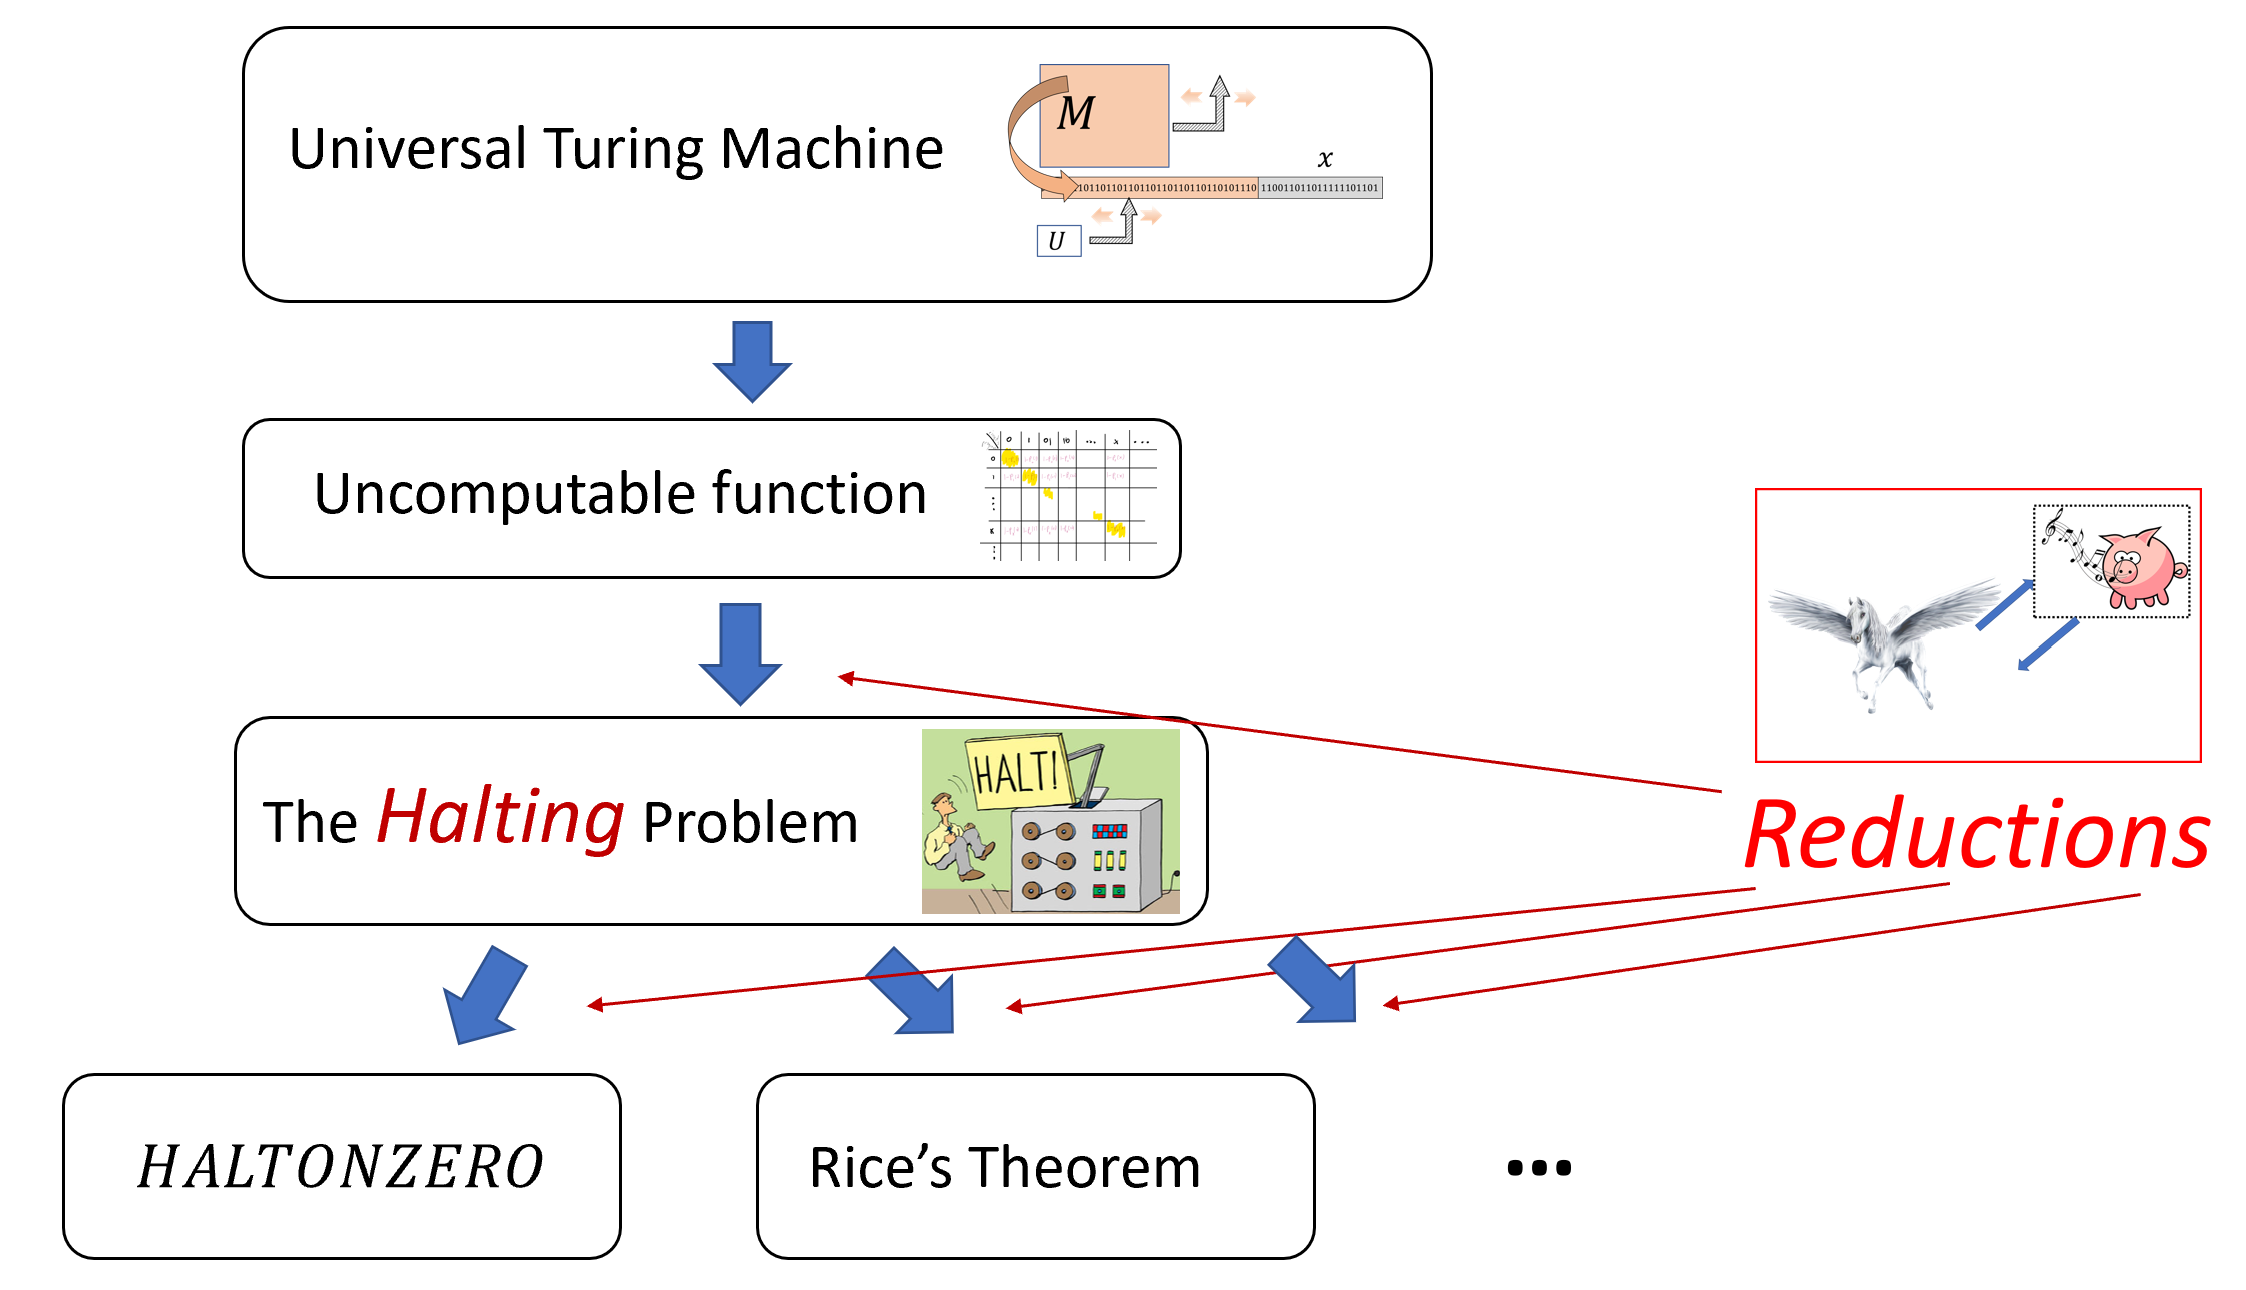
\includegraphics[width=\textwidth, height=0.25\paperheight, keepaspectratio]{../figure/universalchapoverview.png}
\caption{In this chapter we will show the existence of a \emph{universal
Turing machine} and then use this to derive first the existence of
\emph{some} uncomputable function. We then use this to derive the
uncomputability of Turing's famous ``halting problem'' (i.e., the
\(\ensuremath{\mathit{HALT}}\) function), from which we a host of other
uncomputability results follow. We also introduce \emph{reductions},
which allow us to use the uncomputability of a function \(F\) to derive
the uncomputability of a new function \(G\).}
\label{universalchapoverviewfig}
\end{figure}

\section{Universality or a meta-circular
evaluator}\label{Universality-or-a-meta-ci}

We start by proving the existence of a \emph{universal Turing machine}.
This is a single Turing machine \(U\) that can evaluate \emph{arbitrary}
Turing machines \(M\) on \emph{arbitrary} inputs \(x\), including
machines \(M\) that can have more states and larger alphabet than \(U\)
itself. In particular, \(U\) can even be used to evaluate itself! This
notion of \emph{self reference} will appear time and again in this
course, and as we will see, leads to several counter-intuitive phenomena
in computing.

\hypertarget{universaltmthm}{}
\begin{theorem}[Universal Turing Machine] \label[theorem]{universaltmthm}

There exists a Turing machine \(U\) such that on every string \(M\)
which represents a Turing machine, and \(x\in \{0,1\}^*\),
\(U(M,x)=M(x)\).

That is, if the machine \(M\) halts on \(x\) and outputs some
\(y\in \{0,1\}^*\) then \(U(M,x)=y\), and if \(M\) does not halt on
\(x\) (i.e., \(M(x)=\bot\)) then \(U(M,x)=\bot\).

\end{theorem}


\begin{marginfigure}
\centering
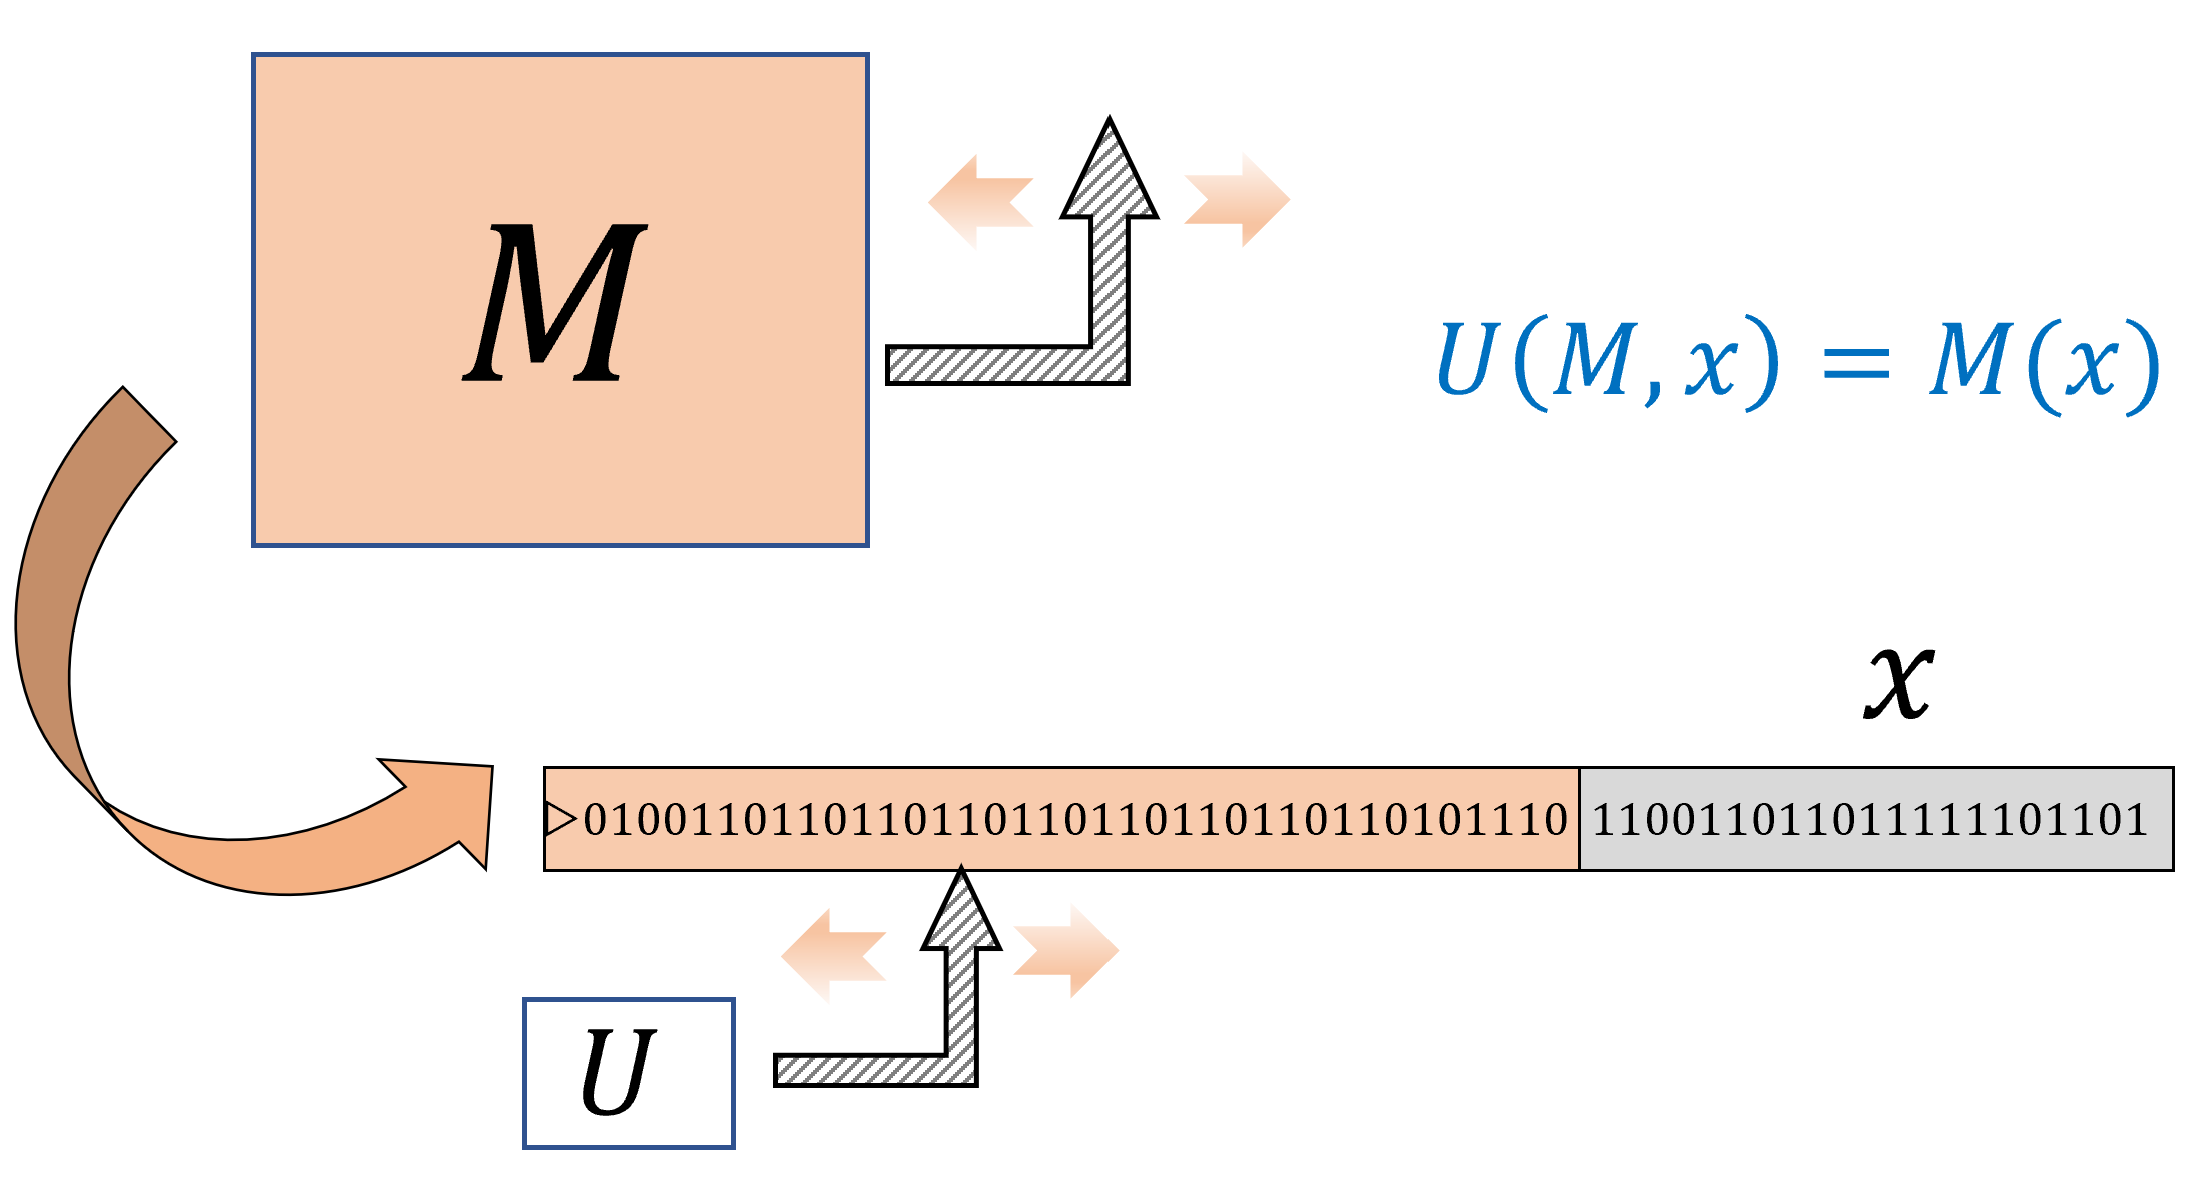
\includegraphics[width=\linewidth, height=1.5in, keepaspectratio]{../figure/universaltm.png}
\caption{A \emph{Universal Turing Machine} is a single Turing Machine
\(U\) that can evaluate, given input the (description as a string of)
arbitrary Turing machine \(M\) and input \(x\), the output of \(M\) on
\(x\). In contrast to the universal circuit depicted in
\cref{universalcircfig}, the machine \(M\) can be much more complex
(e.g., more states or tape alphabet symbols) than \(U\).}
\label{universaltmfig}
\end{marginfigure}

\hypertarget{universaltmidea}{}
\begin{bigidea} \label[bigidea]{universaltmidea}

There is a \emph{``universal''} algorithm that can evaluate arbitrary
algorithms on arbitrary inputs.

\end{bigidea}

\begin{proofidea} \label[proofidea]{Once-you-understand-what-}

Once you understand what the theorem says, it is not that hard to prove.
The desired program \(U\) is an \emph{interpreter} for Turing machines.
That is, \(U\) gets a representation of the machine \(M\) (think of it
as source code), and some input \(x\), and needs to simulate the
execution of \(M\) on \(x\).

Think of how you would code \(U\) in your favorite programming language.
First, you would need to decide on some representation scheme for \(M\).
For example, you can use an array or a dictionary to encode \(M\)'s
transition function. Then you would use some data structure, such as a
list, to store the contents of \(M\)'s tape. Now you can simulate \(M\)
step by step, updating the data structure as you go along. The
interpreter will continue the simulation until the machine halts.

Once you do that, translating this interpreter from your favorite
programming language to a Turing machine can be done just as we have
seen in \cref{chapequivalentmodels}. The end result is what's known as a
``meta-circular evaluator'': an interpreter for a programming language
in the same one. This is a concept that has a long history in computer
science starting from the original universal Turing machine. See also
\cref{lispinterpreterfig}.

\end{proofidea}

\subsection{Proving the existence of a universal Turing
Machine}\label{representtmsec}

To prove (and even properly state) \cref{universaltmthm}, we need to fix
some representation for Turing machines as strings. For example, one
potential choice for such a representation is to use the equivalence
betwen Turing machines and NAND-TM programs and hence represent a Turing
machine \(M\) using the ASCII encoding of the source code of the
corresponding NAND-TM program \(P\). However, we will use a more direct
encoding.

\hypertarget{representTM}{}
\begin{definition}[String representation of Turing Machine] \label[definition]{representTM}

Let \(M\) be a Turing machine with \(k\) states and a size \(\ell\)
alphabet \(\Sigma = \{ \sigma_0,\ldots,\sigma_{\ell-1} \}\) (we use the
convention \(\sigma_0 = 0\),\(\sigma_1 = 1\),
\(\sigma_2 = \varnothing\), \(\sigma_3=\triangleright\)). We represent
\(M\) as the triple \((k,\ell,T)\) where \(T\) is the table of values
for \(\delta_M\):

\[T = \left(\delta_M(0,0),\delta_M(0,\sigma_0),\ldots,\delta_M(k-1,\sigma_{k-1})\right) \;,\]

where each value \(\delta_M(s,\sigma)\) is a triple \((s',\sigma',d)\)
with \(s'\in [k]\), \(\sigma'\in \Sigma\) and \(d\) a number
\(\{0,1,2,3 \}\) encoding one of
\(\{ \mathsf{L},\mathsf{R},\mathsf{S},\mathsf{H} \}\). Thus such a
machine \(M\) is encoded by a list of \(2 + 3k\cdot\ell\) natural
numbers. The \emph{string representation} of \(M\) is obtained by
concatenating prefix free representation of all these integers. If a
string \(\alpha \in \{0,1\}^*\) does not represent a list of integers in
the form above, then we treat it as representing the trivial Turing
machine with one state that immediately halts on every input.

\end{definition}

\hypertarget{TMrepremark}{}
\begin{remark}[Take away points of representation] \label[remark]{TMrepremark}

The details of the representation scheme of Turing machines as strings
are immaterial for almost all applications. What you need to remember
are the following points:

\begin{enumerate}
\def\labelenumi{\arabic{enumi}.}
\item
  We can represent every Turing machine as a string.
\item
  Given the string representation of a Turing machine \(M\) and an input
  \(x\), we can simulate \(M\)'s execution on the input \(x\). (This is
  the content of \cref{universaltmthm}.)
\end{enumerate}

An additional minor issue is that for convenience we make the assumption
that \emph{every} string represents \emph{some} Turing machine. This is
very easy to ensure by just mapping strings that would otherwise not
represent a Turing machine into some fixed trivial machine. This
assumption is not very important, but does make a few results (such as
Rice's Theorem: \cref{rice-thm}) a little less cumbersome to state.

\end{remark}

Using this representation, we can formally prove \cref{universaltmthm}.

\begin{proof}[Proof of \cref{universaltmthm}] \label[proof]{We-will-only-sketch-the-p}

We will only sketch the proof, giving the major ideas. First, we observe
that we can easily write a \emph{Python} program that, on input a
representation \((k,\ell,T)\) of a Turing machine \(M\) and an input
\(x\), evaluates \(M\) on \(X\). Here is the code of this program for
concreteness, though you can feel free to skip it if you are not
familiar with (or interested in) Python:

\begin{code}
# constants
def EVAL(δ,x):
    '''Evaluate TM given by transition table δ
    on input x'''
    Tape = ["▷"] + [a for a in x]
    i = 0; s = 0 # i = head pos, s = state
    while True:
        s, Tape[i], d = δ[(s,Tape[i])]
        if d == "H": break
        if d == "L": i = max(i-1,0)
        if d == "R": i += 1
        if i>= len(Tape): Tape.append('Φ')

    j = 1; Y = [] # produce output
    while Tape[j] != 'Φ':
        Y.append(Tape[j])
        j += 1
    return Y
\end{code}

On input a transition table \(\delta\) this program will simulate the
corresponding machine \(M\) step by step, at each point maintaining the
invariant that the array \texttt{Tape} contains the contents of \(M\)'s
tape, and the variable \texttt{s} contains \(M\)'s current state.

The above does not prove the theorem as stated, since we need to show a
\emph{Turing machine} that computes \(\ensuremath{\mathit{EVAL}}\)
rather than a Python program. With enough effort, we can translate this
Python code line by line to a Turing machine. However, to prove the
theorem we don't need to do this, but can use our ``eat the cake and
have it too'' paradigm. That is, while we need to evaluate a Turing
machine, in writing the code for the interpreter we are allowed to use a
richer model such as NAND-RAM since it is equivalent in power to Turing
machines per \cref{RAMTMequivalencethm}).

Translating the above Python code to NAND-RAM is truly straightforward.
The only issue is that NAND-RAM doesn't have the \emph{dictionary} data
structure built in, which we have used above to store the transition
function \texttt{δ}. However, we can represent a dictionary \(D\) of the
form \(\{ key_0:val_0 , \ldots, key_{m-1}:val_{m-1} \}\) as simply a
list of pairs. To compute \(D[k]\) we can scan over all the pairs until
we find one of the form \((k,v)\) in which case we return \(v\).
Similarly we scan the list to update the dictionary with a new value,
either modifying it or appending the pair \((key,val)\) at the end.

\end{proof}

\begin{remark}[Efficiency of the simulation] \label[remark]{The-argument-in-the-proof}

The argument in the proof of \cref{universaltmthm} is a very inefficient
way to implement the dictionary data structure in practice, but it
suffices for the purpose of proving the theorem. Reading and writing to
a dictionary of \(m\) values in this implementation takes \(\Omega(m)\)
steps, but it is in fact possible to do this in \(O(\log m)\) steps
using a \emph{search tree} data structure or even \(O(1)\) (for
``typical'' instances) using a \emph{hash table}. NAND-RAM and RAM
machines correspond to the architecture of modern electronic computers,
and so we can implement hash tables and search trees in NAND-RAM just as
they are implemented in other programming languages.

\end{remark}

\hypertarget{directunivtm}{}
\begin{remark}[Direct construction of universal Turing Machines] \label[remark]{directunivtm}

Since universal Turing

\end{remark}

\subsection{Implications of universality
(discussion)}\label{Implications-of-universal}


\begin{figure}
\centering
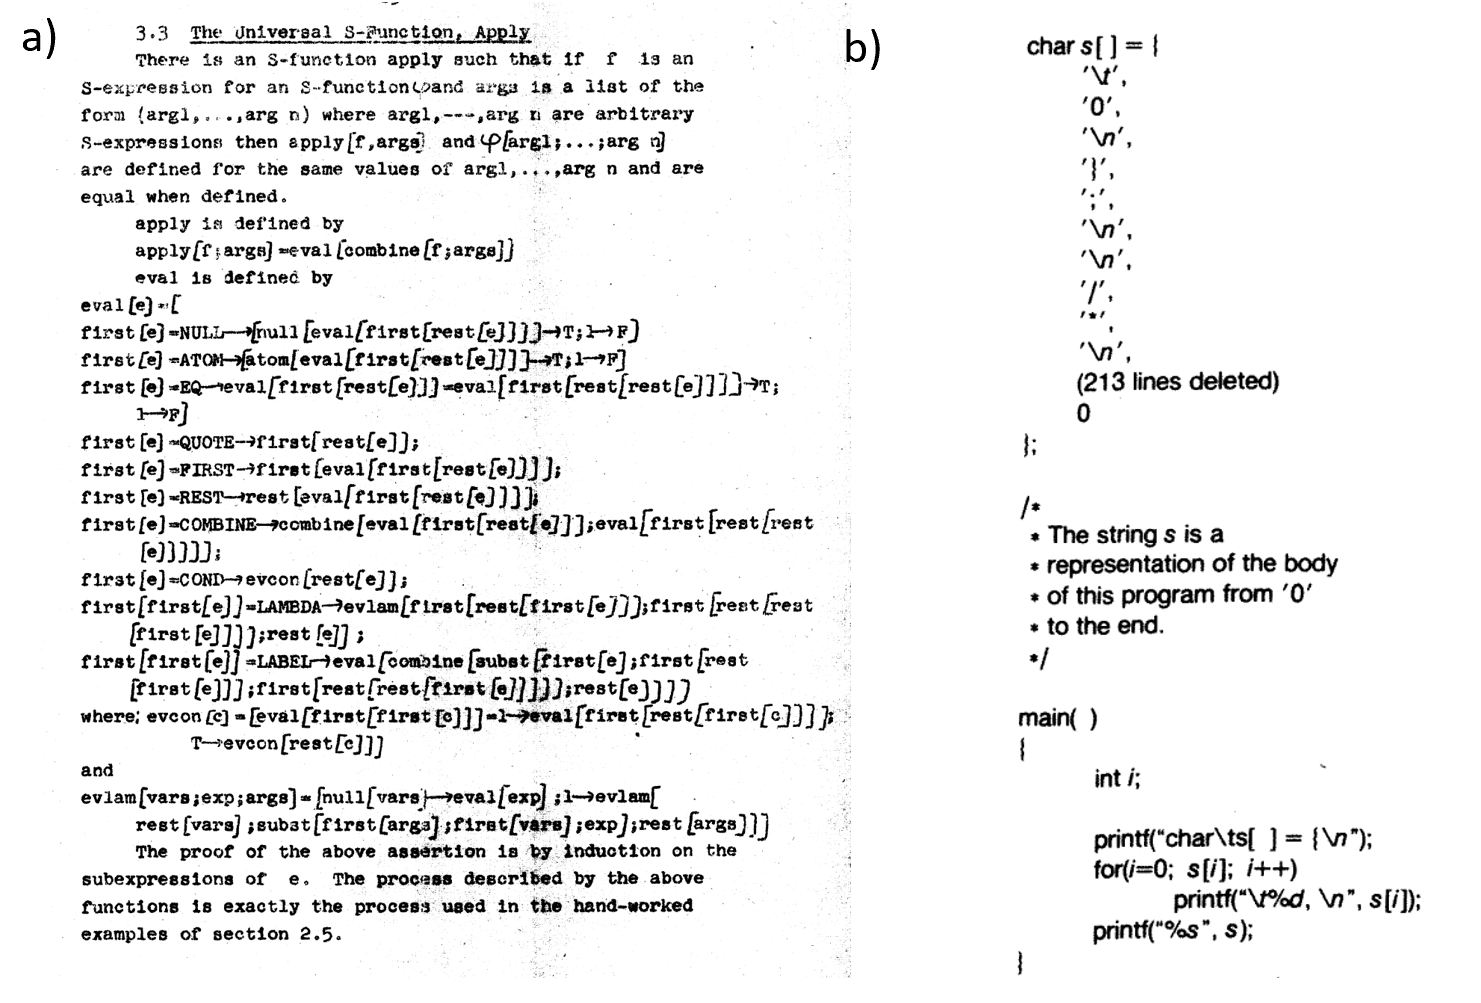
\includegraphics[width=\textwidth, height=0.25\paperheight, keepaspectratio]{../figure/lispandselfreplicatingprograms.png}
\caption{\textbf{a)} A particularly elegant example of a ``meta-circular
evaluator'' comes from John McCarthy's 1960 paper, where he defined the
Lisp programming language and gave a Lisp function that evaluates an
arbitrary Lisp program (see above). Lisp was not initially intended as a
practical programming language and this example was merely meant as an
illustration that the Lisp universal function is more elegant than the
universal Turing machine. It was McCarthy's graduate student Steve
Russell who suggested that it can be implemented. As McCarthy later
recalled, \emph{``I said to him, ho, ho, you're confusing theory with
practice, this eval is intended for reading, not for computing. But he
went ahead and did it. That is, he compiled the eval in my paper into
IBM 704 machine code, fixing a bug, and then advertised this as a Lisp
interpreter, which it certainly was''.} \textbf{b)} A self-replicating C
program from the classic essay of Thompson
\cite{thompson1984reflections}.}
\label{lispinterpreterfig}
\end{figure}

There is more than one Turing machine \(U\) that satisfies the
conditions of \cref{universaltmthm}, but the existence of even a single
such machine is already extremely fundamental to both the theory and
practice of computer science. \cref{universaltmthm}'s impact reaches
beyond the particular model of Turing machines. Because we can simulate
every Turing Machine by a NAND-TM program and vice versa,
\cref{universaltmthm} immediately implies there exists a universal
NAND-TM program \(P_U\) such that \(P_U(P,x)=P(x)\) for every NAND-TM
program \(P\). We can also ``mix and match'' models. For example since
we can simulate every NAND-RAM program by a Turing machine, and every
Turing Machine by the \(\lambda\) calculus, \cref{universaltmthm}
implies that there exists a \(\lambda\) expression \(e\) such that for
every NAND-RAM program \(P\) and input \(x\) on which \(P(x)=y\), if we
encode \((P,x)\) as a \(\lambda\)-expression \(f\) (using the
\(\lambda\)-calculus encoding of strings as lists of \(0\)'s and
\(1\)'s) then \((e\; f)\) evaluates to an encoding of \(y\). More
generally we can say that for every \(\mathcal{X}\) and \(\mathcal{Y}\)
in the set \(\{\) Turing Machines, RAM Machines, NAND-TM, NAND-RAM,
\(\lambda\)-calculus, JavaScript, Python, \(\ldots\) \(\}\) of Turing
equivalent models, there exists a program/machine in \(\mathcal{X}\)
that computes the map \((P,x) \mapsto P(x)\) for every program/machine
\(P \in \mathcal{Y}\).

The idea of a ``universal program'' is of course not limited to theory.
For example compilers for programming languages are often used to
compile \emph{themselves}, as well as programs more complicated than the
compiler. (An extreme example of this is Fabrice Bellard's
\href{https://bellard.org/otcc/}{Obfuscated Tiny C Compiler} which is a
C program of 2048 bytes that can compile a large subset of the C
programming language, and in particular can compile itself.) This is
also related to the fact that it is possible to write a program that can
print its own source code, see \cref{lispinterpreterfig}. There are
universal Turing machines known that require a very small number of
states or alphabet symbols, and in particular there is a universal
Turing machine (with respect to a particular choice of representing
Turing machines as strings) whose tape alphabet is
\(\{ \triangleright, \varnothing, 0, 1 \}\) and has fewer than \(25\)
states (see \cref{uncomputablebibnotes}).

\section{Is every function computable?}\label{Is-every-function-computa}

In \cref{NAND-univ-thm}, we saw that NAND-CIRC programs can compute
every finite function \(f:\{0,1\}^n \rightarrow \{0,1\}\). Therefore a
natural guess is that NAND-TM programs (or equivalently, Turing
Machines) could compute every infinite function
\(F:\{0,1\}^* \rightarrow \{0,1\}\). However, this turns out to be
\emph{false}. That is, there exists a function
\(F:\{0,1\}^* \rightarrow \{0,1\}\) that is \emph{uncomputable}!

The existence of uncomputable functions is quite surprising. Our
intuitive notion of a ``function'' (and the notion most mathematicians
had until the 20th century) is that a function \(f\) defines some
implicit or explicit way of computing the output \(f(x)\) from the input
\(x\). The notion of an ``uncomputable function'' thus seems to be a
contradiction in terms, but yet the following theorem shows that such
creatures do exist:

\hypertarget{uncomputable-func}{}
\begin{theorem}[Uncomputable functions] \label[theorem]{uncomputable-func}

There exists a function \(F^*:\{0,1\}^* \rightarrow \{0,1\}\) that is
not computable by any Turing machine.

\end{theorem}

\begin{proofidea} \label[proofidea]{The-idea-behind-the-proof}

The idea behind the proof follows quite closely Cantor's proof that the
reals are uncountable (\cref{cantorthm}), and in fact the theorem can
also be obtained fairly directly from that result (see
\cref{uncountablefuncex}). However, it is instructive to see the direct
proof. The idea is to construct \(F^*\) in a way that will ensure that
every possible machine \(M\) will in fact fail to compute \(F^*\). We do
so by defining \(F^*(x)\) to equal \(0\) if \(x\) describes a Turing
machine \(M\) which satisfies \(M(x)=1\) and defining \(F^*(x)=1\)
otherwise. By construction, if \(M\) is any Turing machine and \(x\) is
the string describing it, then \(F^*(x) \neq M(x)\) and therefore \(M\)
does \emph{not} compute \(F^*\).

\end{proofidea}

\begin{proof}[Proof of \cref{uncomputable-func}] \label[proof]{The-proof-is-illustrated-}

The proof is illustrated in \cref{diagonal-fig}. We start by defining
the following function \(G:\{0,1\}^* \rightarrow \{0,1\}\):

For every string \(x\in\{0,1\}^*\), if \(x\) satisfies \textbf{(1)}
\(x\) is a valid representation of some Turing machine \(M\) (per the
representation scheme above) and \textbf{(2)} when the program \(M\) is
executed on the input \(x\) it halts and produces an output, then we
define \(G(x)\) as the first bit of this output. Otherwise (i.e., if
\(x\) is not a valid representation of a Turing machine, or the machine
\(M_x\) never halts on \(x\)) we define \(G(x)=0\). We define
\(F^*(x) = 1 - G(x)\).

We claim that there is no Turing machine that computes \(F^*\). Indeed,
suppose, towards the sake of contradiction, there exists a machine \(M\)
that computes \(F^*\), and let \(x\) be the binary string that
represents the machine \(M\). On one hand, since by our assumption \(M\)
computes \(F^*\), on input \(x\) the machine \(M\) halts and outputs
\(F^*(x)\). On the other hand, by the definition of \(F^*\), since \(x\)
is the representation of the machine \(M\),
\(F^*(x) = 1 - G(x) = 1 - M(x)\), hence yielding a contradiction.

\end{proof}


\begin{figure}
\centering
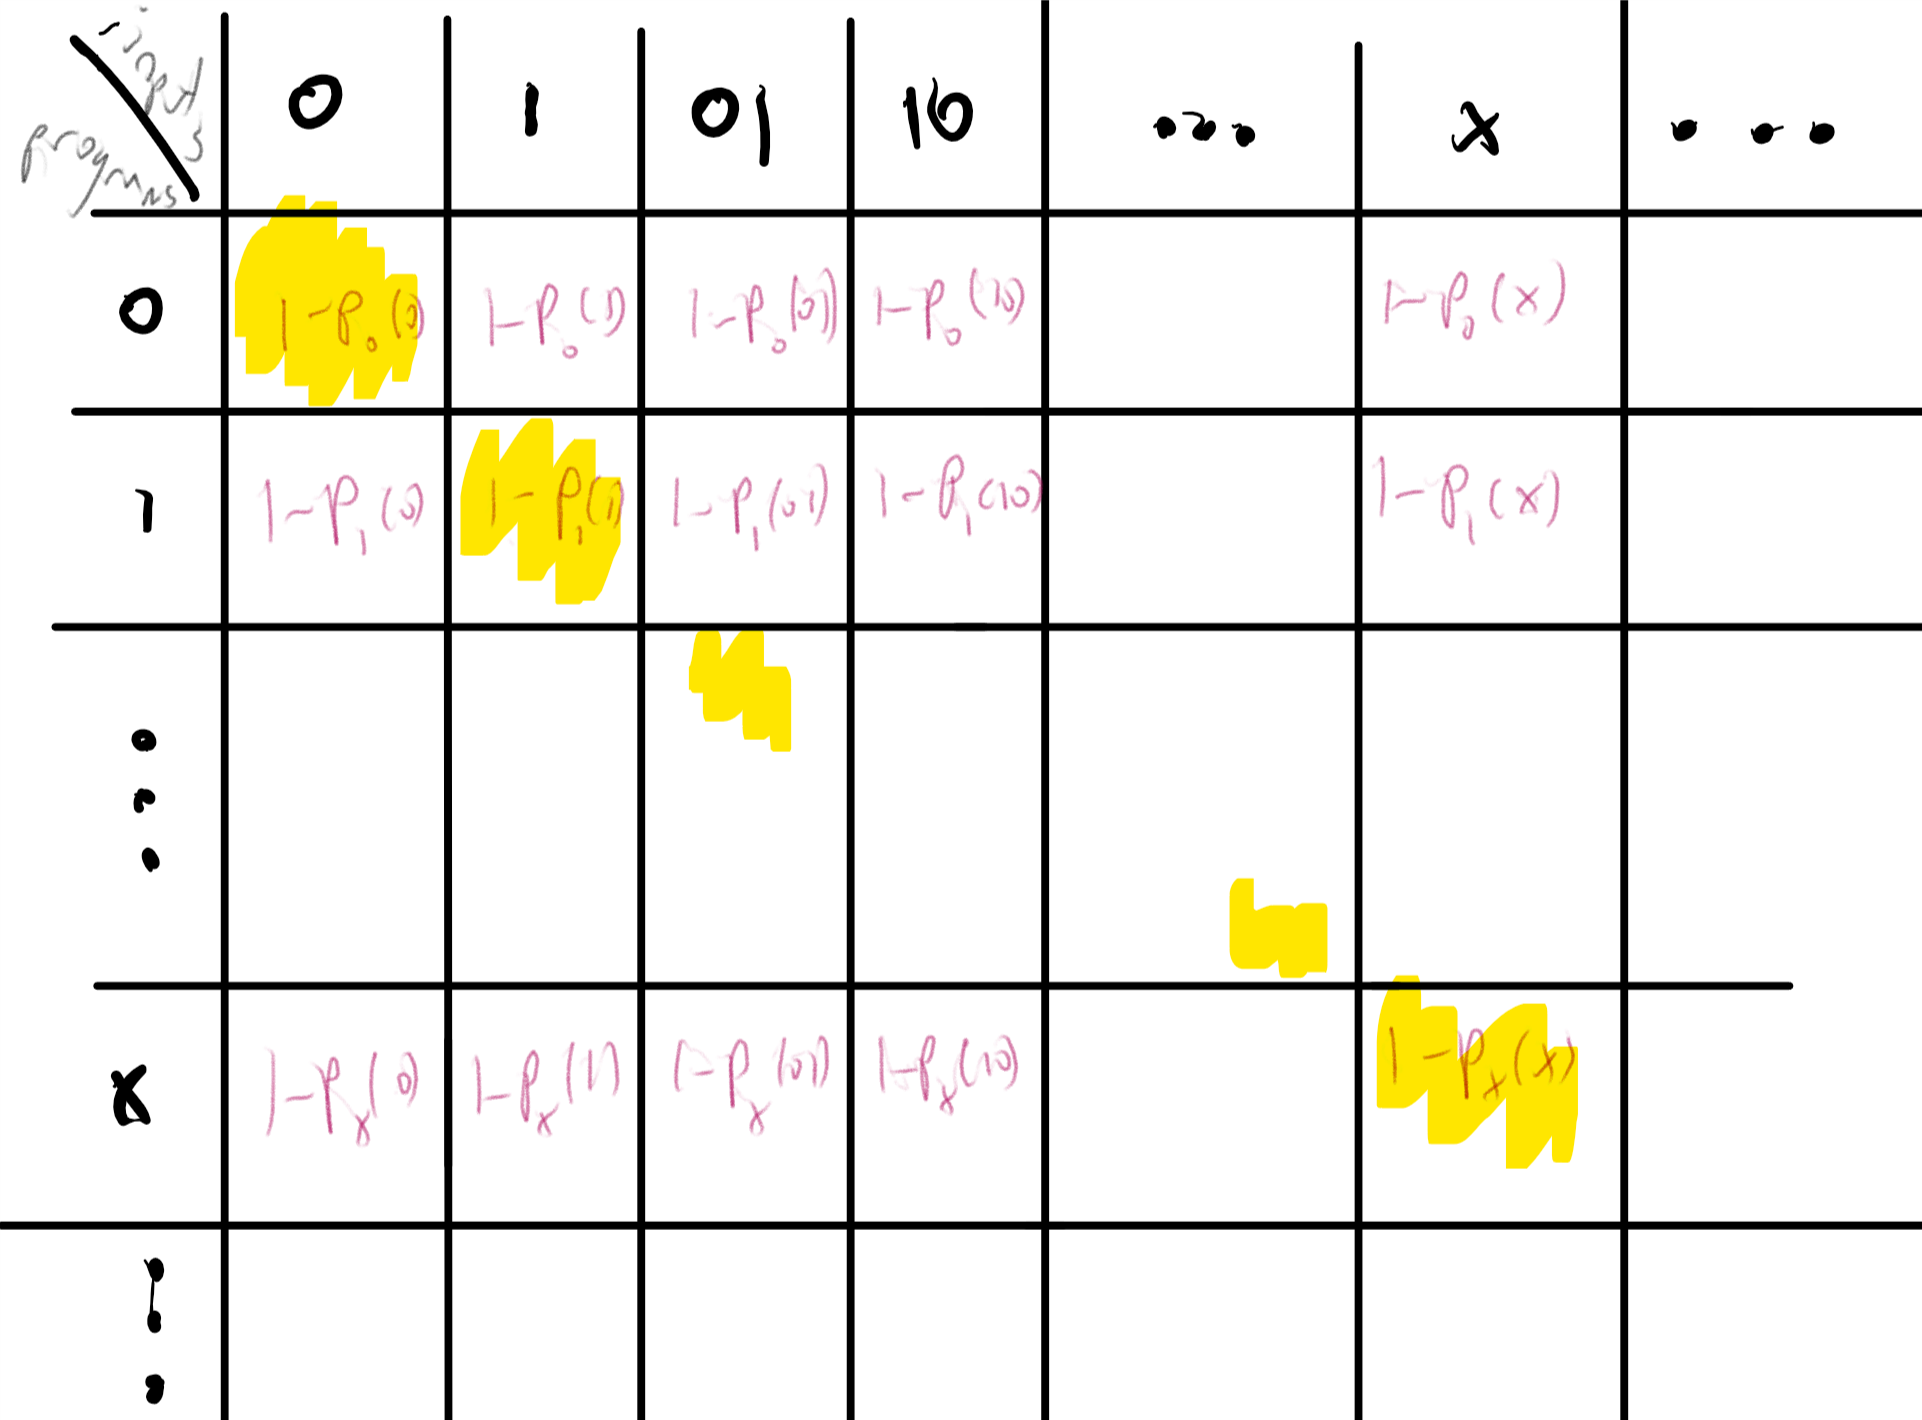
\includegraphics[width=\textwidth, height=0.25\paperheight, keepaspectratio]{../figure/diagonal_proof.png}
\caption{We construct an uncomputable function by defining for every two
strings \(x,y\) the value \(1-M_y(x)\) which equals \(0\) if the machine
described by \(y\) outputs \(1\) on \(x\), and \(1\) otherwise. We then
define \(F^*(x)\) to be the ``diagonal'' of this table, namely
\(F^*(x)=1-M_x(x)\) for every \(x\). The function \(F^*\) is
uncomputable, because if it was computable by some machine whose string
description is \(x^*\) then we would get that
\(M_{x^*}(x^*)=F(x^*)=1-M_{x^*}(x^*)\).}
\label{diagonal-fig}
\end{figure}

\hypertarget{uncomputablefunctions}{}
\begin{bigidea} \label[bigidea]{uncomputablefunctions}

There are some functions that \emph{can not} be computed by \emph{any}
algorithm.

\end{bigidea}

\begin{pause} \label[pause]{The-proof-of-crefuncomput}

The proof of \cref{uncomputable-func} is short but subtle. I suggest
that you pause here and go back to read it again and think about it -
this is a proof that is worth reading at least twice if not three or
four times. It is not often the case that a few lines of mathematical
reasoning establish a deeply profound fact - that there are problems we
simply \emph{cannot} solve.

\end{pause}

The type of argument used to prove \cref{uncomputable-func} is known as
\emph{diagonalization} since it can be described as defining a function
based on the diagonal entries of a table as in \cref{diagonal-fig}. The
proof can be thought of as an infinite version of the \emph{counting}
argument we used for showing lower bound for NAND-CIRC programs in
\cref{counting-lb}. Namely, we show that it's not possible to compute
all functions from \(\{0,1\}^* \rightarrow \{0,1\}\) by Turing machines
simply because there are more functions like that then there are Turing
machines.

As mentioned in \cref{decidablelanguages}, many texts use the
``language'' terminology and so will call a set
\(L \subseteq \{0,1\}^*\) an
\href{https://goo.gl/3YvQvL}{\emph{undecidable}} or \emph{non recursive}
language if the function \(F:\{0,1\}^* :\rightarrow \{0,1\}\) such that
\(F(x)=1 \leftrightarrow x\in L\) is uncomputable.

\section{The Halting problem}\label{haltingsec}

\cref{uncomputable-func} shows that there is \emph{some} function that
cannot be computed. But is this function the equivalent of the ``tree
that falls in the forest with no one hearing it''? That is, perhaps it
is a function that no one actually \emph{wants} to compute. It turns out
that there are natural uncomputable functions:

\hypertarget{halt-thm}{}
\begin{theorem}[Uncomputability of Halting function] \label[theorem]{halt-thm}

Let \(\ensuremath{\mathit{HALT}}:\{0,1\}^* \rightarrow \{0,1\}\) be the
function such that for every string \(M\in \{0,1\}^*\),
\(\ensuremath{\mathit{HALT}}(M,x)=1\) if Turing machine \(M\) halts on
the input \(x\) and \(\ensuremath{\mathit{HALT}}(M,x)=0\) otherwise.
Then \(\ensuremath{\mathit{HALT}}\) is not computable.

\end{theorem}

Before turning to prove \cref{halt-thm}, we note that
\(\ensuremath{\mathit{HALT}}\) is a very natural function to want to
compute. For example, one can think of \(\ensuremath{\mathit{HALT}}\) as
a special case of the task of managing an ``App store''. That is, given
the code of some application, the gatekeeper for the store needs to
decide if this code is safe enough to allow in the store or not. At a
minimum, it seems that we should verify that the code would not go into
an infinite loop.

\begin{proofidea} \label[proofidea]{One-way-to-think-about-th}

One way to think about this proof is as follows: \[
\text{Uncomputability of $F^*$} \;+\; \text{Universality} \;=\; \text{Uncomputability of $\ensuremath{\mathit{HALT}}$}
\] That is, we will use the universal Turing machine that computes
\(\ensuremath{\mathit{EVAL}}\) to derive the uncomputability of
\(\ensuremath{\mathit{HALT}}\) from the uncomputability of \(F^*\) shown
in \cref{uncomputable-func}. Specifically, the proof will be by
contradiction. That is, we will assume towards a contradiction that
\(\ensuremath{\mathit{HALT}}\) is computable, and use that assumption,
together with the universal Turing machine of \cref{universaltmthm}, to
derive that \(F^*\) is computable, which will contradict
\cref{uncomputable-func}.

\end{proofidea}

\hypertarget{reductionuncomputeidea}{}
\begin{bigidea} \label[bigidea]{reductionuncomputeidea}

If a function \(F\) is uncomputable we can show that another function
\(H\) is uncomputable by giving a way to \emph{reduce} the task of
computing \(F\) to computing \(H\).

\end{bigidea}

\begin{proof}[Proof of \cref{halt-thm}] \label[proof]{The-proof-will-use-the-pr}

The proof will use the previously established result
\cref{uncomputable-func}. Recall that \cref{uncomputable-func} shows
that the following function \(F^*: \{0,1\}^* \rightarrow \{0,1\}\) is
uncomputable:

\[
F^*(x) = \begin{cases}1 & x(x)=0 \\ 0 & \text{otherwise} \end{cases}
\] where \(x(x)\) denotes the output of the Turing machine described by
the string \(x\) on the input \(x\) (with the usual convention that
\(x(x)=\bot\) if this computation does not halt).

We will show that the uncomputability of \(F^*\) implies the
uncomputability of \(\ensuremath{\mathit{HALT}}\). Specifically, we will
assume, towards a contradiction, that there exists a Turing machine
\(M\) that can compute the \(\ensuremath{\mathit{HALT}}\) function, and
use that to obtain a Turing machine \(M'\) that computes the function
\(F^*\). (This is known as a proof by \emph{reduction}, since we reduce
the task of computing \(F^*\) to the task of computing
\(\ensuremath{\mathit{HALT}}\). By the contrapositive, this means the
uncomputability of \(F^*\) implies the uncomputability of
\(\ensuremath{\mathit{HALT}}\).)

Indeed, suppose that \(M\) is a Turing machine that computes
\(\ensuremath{\mathit{HALT}}\). \cref{halttof} describes a Turing
Machine \(M'\) that computes \(F^*\). (We use ``high level'' description
of Turing machines, appealing to the ``have your cake and eat it too''
paradigm, see \cref{eatandhavecake}.)

\begin{algorithm}[$F^*$ to $HALT$ reduction]
\label[algorithm]{halttof} ~ \\ \noindent
\begin{algorithmic}[1]
\INPUT  $x\in \{0,1\}^*$
\OUTPUT  $F^*(x)$
\STATE \COMMENT{ Assume T.M. $M_{HALT}$ computes $HALT$}
\STATE Let $z \leftarrow M_{HALT}(x,x)$. \COMMENT{ Assume $z=HALT(x,x)$.}
\IF{$z=0$}
\RETURN $0$
\ENDIF
\STATE Let $y \leftarrow U(x,x)$ \COMMENT{ $U$ universal TM, i.e., $y=x(x)$}
\IF{$y=0$}
\RETURN $1$
\ENDIF
\RETURN $0$
\end{algorithmic}
\end{algorithm}

We claim that \cref{halttof} computes the function \(F^*\). Indeed,
suppose that \(x(x)=0\) (and hence \(F^*(x)=1\)). In this case,
\(\ensuremath{\mathit{HALT}}(x,x)=1\) and hence, under our assumption
that \(M(x,x)=\ensuremath{\mathit{HALT}}(x,x)\), the value \(z\) will
equal \(1\), and hence \cref{halttof} will set \(y=x(x)=0\), and output
the correct value \(1\).

Suppose otherwise that \(x(x) \neq 0\) (and hence \(F^*(x)=0\)). In this
case there are two possibilities:

\begin{itemize}
\item
  \textbf{Case 1:} The machine described by \(x\) does not halt on the
  input \(x\). In this case, \(\ensuremath{\mathit{HALT}}(x,x)=0\).
  Since we assume that \(M\) computes \(\ensuremath{\mathit{HALT}}\) it
  means that on input \(x,x\), the machine \(M\) must halt and output
  the value \(0\). This means that \cref{halttof} will set \(z=0\) and
  output \(0\).
\item
  \textbf{Case 2:} The machine described by \(x\) halts on the input
  \(x\) and outputs some \(y' \neq 0\). In this case, since
  \(\ensuremath{\mathit{HALT}}(x,x)=1\), under our assumptions,
  \cref{halttof} will set \(y=y' \neq 0\) and so output \(0\).
\end{itemize}

We see that in all cases, \(M'(x)=F^*(x)\), which contradicts the fact
that \(F^*\) is uncomputable. Hence we reach a contradiction to our
original assumption that \(M\) computes \(\ensuremath{\mathit{HALT}}\).

\end{proof}

\begin{pause} \label[pause]{Once-again-this-is-a-proo}

Once again, this is a proof that's worth reading more than once. The
uncomputability of the halting problem is one of the fundamental
theorems of computer science, and is the starting point for much of the
investigations we will see later. An excellent way to get a better
understanding of \cref{halt-thm} is to go over
\cref{haltalternativesec}, which presents an alternative proof of the
same result.

\end{pause}

\subsection{Is the Halting problem really hard?
(discussion)}\label{Is-the-Halting-problem-re}

Many people's first instinct when they see the proof of \cref{halt-thm}
is to not believe it. That is, most people do believe the mathematical
statement, but intuitively it doesn't seem that the Halting problem is
really that hard. After all, being uncomputable only means that
\(\ensuremath{\mathit{HALT}}\) cannot be computed by a Turing machine.

But programmers seem to solve \(\ensuremath{\mathit{HALT}}\) all the
time by informally or formally arguing that their programs halt. It's
true that their programs are written in C or Python, as opposed to
Turing machines, but that makes no difference: we can easily translate
back and forth between this model and any other programming language.

While every programmer encounters at some point an infinite loop, is
there really no way to solve the halting problem? Some people argue that
\emph{they} personally can, if they think hard enough, determine whether
any concrete program that they are given will halt or not. Some have
even \href{https://goo.gl/Bm4MWK}{argued} that humans in general have
the ability to do that, and hence humans have inherently superior
intelligence to computers or anything else modeled by Turing
machines.\footnote{This argument has also been connected to the issues
  of consciousness and free will. I am personally skeptical of its
  relevance to these issues. Perhaps the reasoning is that humans have
  the ability to solve the halting problem but they exercise their free
  will and consciousness by choosing not to do so.}

The best answer we have so far is that there truly is no way to solve
\(\ensuremath{\mathit{HALT}}\), whether using Macs, PCs, quantum
computers, humans, or any other combination of electronic, mechanical,
and biological devices. Indeed this assertion is the content of the
\emph{Church-Turing Thesis}. This of course does not mean that for
\emph{every} possible program \(P\), it is hard to decide if \(P\)
enters an infinite loop. Some programs don't even have loops at all (and
hence trivially halt), and there are many other far less trivial
examples of programs that we can certify to never enter an infinite loop
(or programs that we know for sure that \emph{will} enter such a loop).
However, there is no \emph{general procedure} that would determine for
an \emph{arbitrary} program \(P\) whether it halts or not. Moreover,
there are some very simple programs for which no one knows whether they
halt or not. For example, the following Python program will halt if and
only if \href{https://goo.gl/DX63q5}{Goldbach's conjecture} is false:

\begin{code}
def isprime(p):
    return all(p % i for i in range(2,p-1))

def Goldbach(n):
    return any( (isprime(p) and isprime(n-p))
           for p in range(2,n-1))

n = 4
while True:
    if not Goldbach(n): break
    n+= 2
\end{code}

Given that Goldbach's Conjecture has been open since 1742, it is unclear
that humans have any magical ability to say whether this (or other
similar programs) will halt or not.


\begin{marginfigure}
\centering
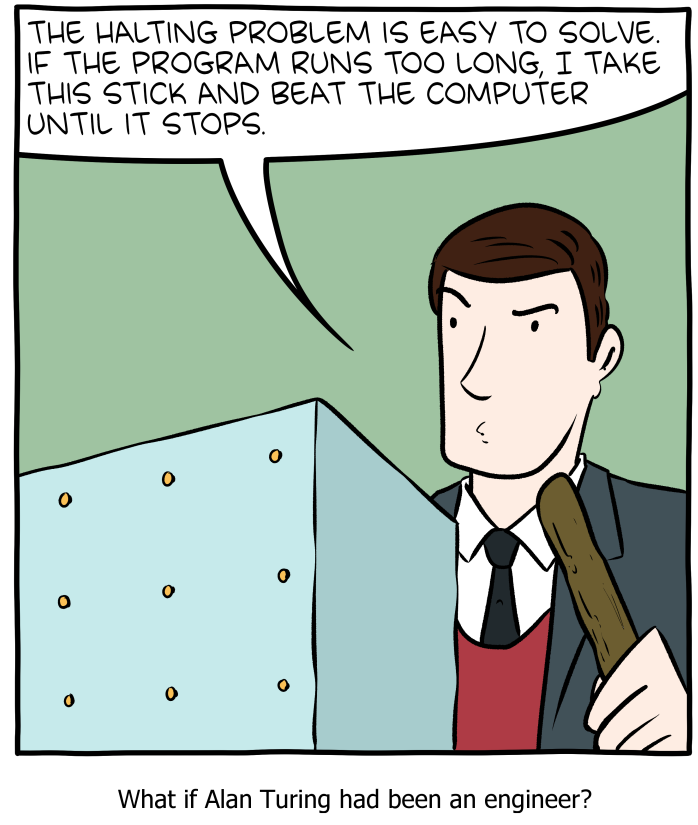
\includegraphics[width=\linewidth, height=1.5in, keepaspectratio]{../figure/smbchalting.png}
\caption{\href{http://smbc-comics.com/comic/halting}{SMBC}'s take on
solving the Halting problem.}
\label{xkcdhaltingfig}
\end{marginfigure}

\subsection{A direct proof of the uncomputability of
\(\ensuremath{\mathit{HALT}}\) (optional)}\label{haltalternativesec}

It turns out that we can combine the ideas of the proofs of
\cref{uncomputable-func} and \cref{halt-thm} to obtain a short proof of
the latter theorem, that does not appeal to the uncomputability of
\(F^*\). This short proof appeared in print in a 1965 letter to the
editor of Christopher Strachey:

\begin{quote}
To the Editor, The Computer Journal.

An Impossible Program

Sir,

A well-known piece of folk-lore among programmers holds that it is
impossible to write a program which can examine any other program and
tell, in every case, if it will terminate or get into a closed loop when
it is run. I have never actually seen a proof of this in print, and
though Alan Turing once gave me a verbal proof (in a railway carriage on
the way to a Conference at the NPL in 1953), I unfortunately and
promptly forgot the details. This left me with an uneasy feeling that
the proof must be long or complicated, but in fact it is so short and
simple that it may be of interest to casual readers. The version below
uses CPL, but not in any essential way.

Suppose \texttt{T[R]} is a Boolean function taking a routine (or
program) \texttt{R} with no formal or free variables as its arguments
and that for all \texttt{R}, \texttt{T[R] = True} if \texttt{R}
terminates if run and that \texttt{T[R] = False} if \texttt{R} does not
terminate.

Consider the routine P defined as follows

\texttt{rec routine P}\\
\texttt{§L: if T[P] go to L}\\
\texttt{Return §}

If \texttt{T[P] = True} the routine \texttt{P} will loop, and it will
only terminate if \texttt{T[P] = False}. In each case `T{[}P{]}`` has
exactly the wrong value, and this contradiction shows that the function
T cannot exist.

Yours faithfully,\\
C. Strachey

Churchill College, Cambridge
\end{quote}

\begin{pause} \label[pause]{Try-to-stop-and-extract-t}

Try to stop and extract the argument for proving \cref{halt-thm} from
the letter above.

\end{pause}

Since CPL is not as common today, let us reproduce this proof. The idea
is the following: suppose for the sake of contradiction that there
exists a program \texttt{T} such that \texttt{T(f,x)} equals
\texttt{True} iff \texttt{f} halts on input \texttt{x}. (Strachey's
letter considers the no-input variant of \(\ensuremath{\mathit{HALT}}\),
but as we'll see, this is an immaterial distinction.) Then we can
construct a program \texttt{P} and an input \texttt{x} such that
\texttt{T(P,x)} gives the wrong answer. The idea is that on input
\texttt{x}, the program \texttt{P} will do the following: run
\texttt{T(x,x)}, and if the answer is \texttt{True} then go into an
infinite loop, and otherwise halt. Now you can see that \texttt{T(P,P)}
will give the wrong answer: if \texttt{P} halts when it gets its own
code as input, then \texttt{T(P,P)} is supposed to be \texttt{True}, but
then \texttt{P(P)} will go into an infinite loop. And if \texttt{P} does
not halt, then \texttt{T(P,P)} is supposed to be \texttt{False} but then
\texttt{P(P)} will halt. We can also code this up in Python:

\begin{code}
def CantSolveMe(T):
    """
    Gets function T that claims to solve HALT.
    Returns a pair (P,x) of code and input on which
    T(P,x) ≠ HALT(x)
    """
    def fool(x):
        if T(x,x):
            while True: pass
        return "I halted"

    return (fool,fool)
\end{code}

For example, consider the following Naive Python program \texttt{T} that
guesses that a given function does not halt if its input contains
\texttt{while} or \texttt{for}

\begin{code}
def T(f,x):
    """Crude halting tester - decides it doesn't halt if it contains a loop."""
    import inspect
    source = inspect.getsource(f)
    if source.find("while"): return False
    if source.find("for"): return False
    return True
\end{code}

If we now set \texttt{(f,x) = CantSolveMe(T)}, then
\texttt{T(f,x)=False} but \texttt{f(x)} does in fact halt. This is of
course not specific to this particular \texttt{T}: for every program
\texttt{T}, if we run \texttt{(f,x) = CantSolveMe(T)} then we'll get an
input on which \texttt{T} gives the wrong answer to
\(\ensuremath{\mathit{HALT}}\).

\section{Reductions}\label{reductionsuncompsec}

The Halting problem turns out to be a linchpin of uncomputability, in
the sense that \cref{halt-thm} has been used to show the uncomputability
of a great many interesting functions. We will see several examples of
such results in this chapter and the exercises, but there are many more
such results (see \cref{haltreductions}).


\begin{figure}
\centering
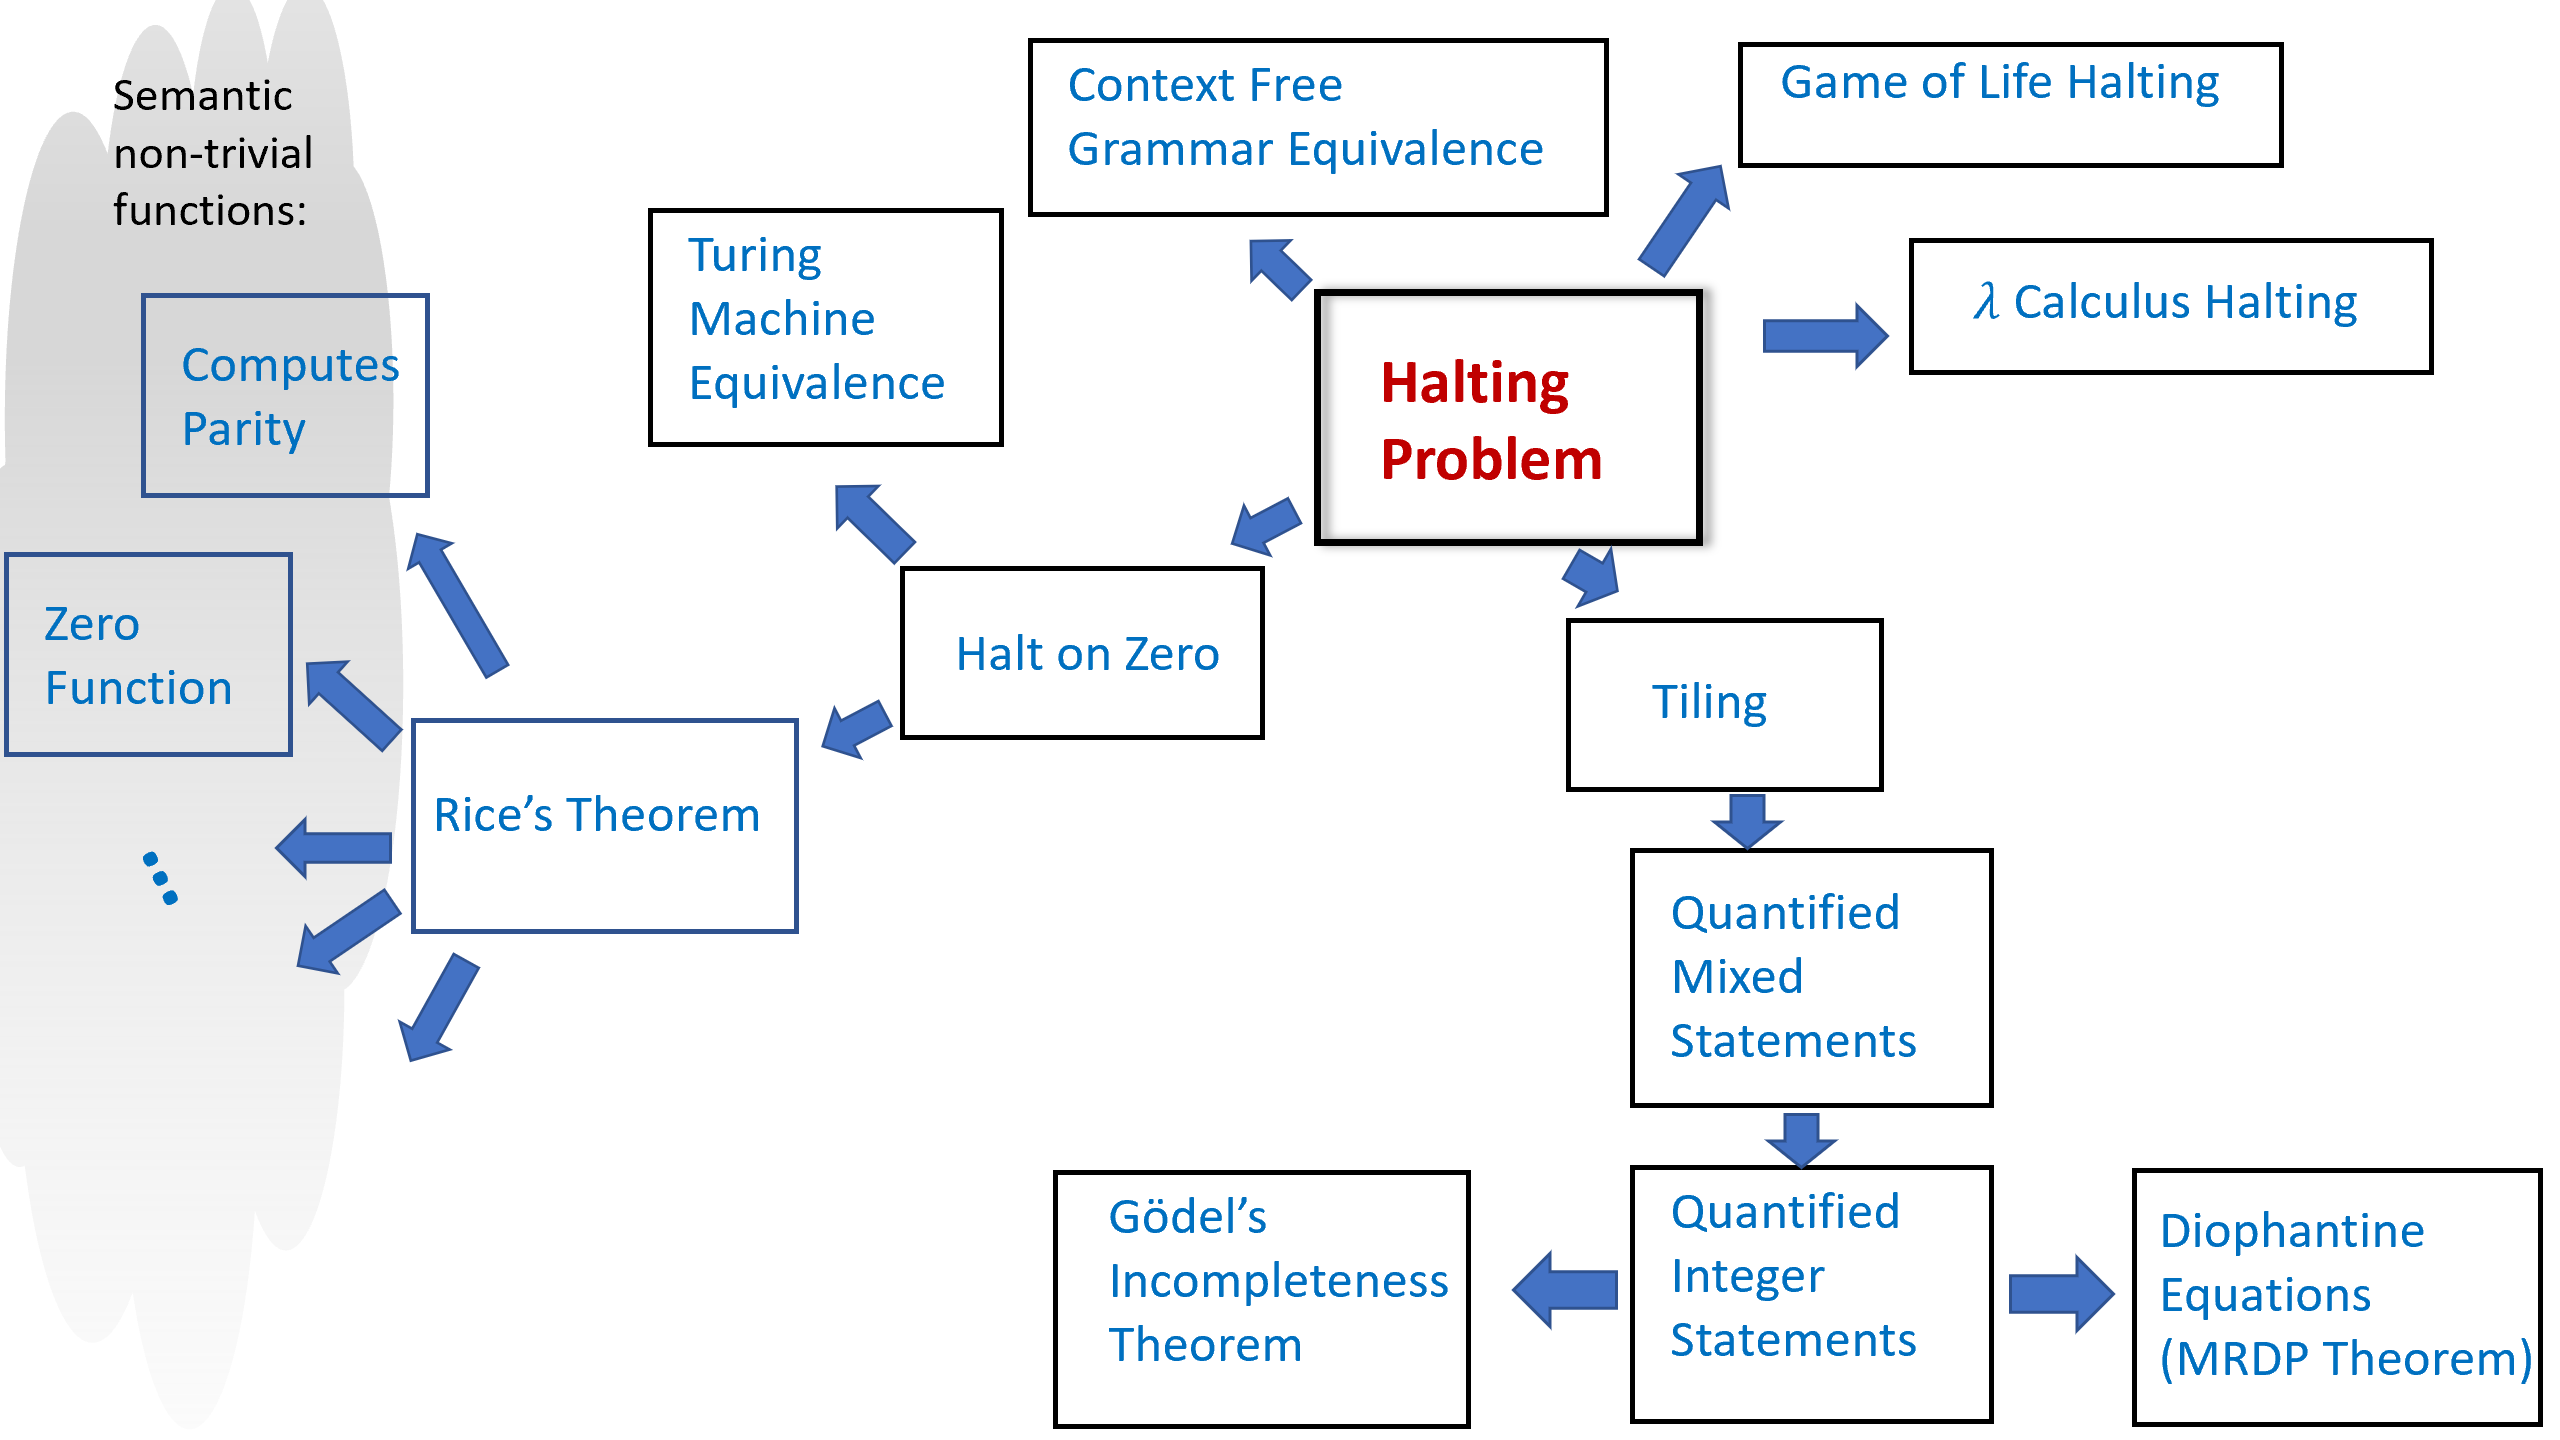
\includegraphics[width=\textwidth, height=0.25\paperheight, keepaspectratio]{../figure/reductions_from_halting.png}
\caption{Some uncomputability results. An arrow from problem X to
problem Y means that we use the uncomputability of X to prove the
uncomputability of Y by reducing computing X to computing Y. All of
these results except for the MRDP Theorem appear in either the text or
exercises. The Halting Problem \(\ensuremath{\mathit{HALT}}\) serves as
our starting point for all these uncomputability results as well as many
others.}
\label{haltreductions}
\end{figure}

The idea behind such uncomputability results is conceptually simple but
can at first be quite confusing. If we know that
\(\ensuremath{\mathit{HALT}}\) is uncomputable, and we want to show that
some other function \(\ensuremath{\mathit{BLAH}}\) is uncomputable, then
we can do so via a \emph{contrapositive} argument (i.e., proof by
contradiction). That is, we show that \textbf{if} there exists a Turing
machine that computes \(\ensuremath{\mathit{BLAH}}\) \textbf{then} there
exists a Turing machine that computes \(\ensuremath{\mathit{HALT}}\).
(Indeed, this is exactly how we showed that
\(\ensuremath{\mathit{HALT}}\) itself is uncomputable, by reducing this
fact to the uncomputability of the function \(F^*\) from
\cref{uncomputable-func}.)

For example, to prove that \(\ensuremath{\mathit{BLAH}}\) is
uncomputable, we could show that there is a computable function
\(R:\{0,1\}^* \rightarrow \{0,1\}^*\) such that for every pair \(M\) and
\(x\),
\(\ensuremath{\mathit{HALT}}(M,x)=\ensuremath{\mathit{BLAH}}(R(M,x))\).
The existence of such a function \(R\) implies that \textbf{if}
\(\ensuremath{\mathit{BLAH}}\) was computable \textbf{then}
\(\ensuremath{\mathit{HALT}}\) would be computable as well, hence
leading to a contradiction! The confusing part about reductions is that
we are assuming something we \emph{believe} is false (that
\(\ensuremath{\mathit{BLAH}}\) has an algorithm) to derive something
that we \emph{know} is false (that \(\ensuremath{\mathit{HALT}}\) has an
algorithm). Michael Sipser describes such results as having the form
\emph{``If pigs could whistle then horses could fly''}.

A reduction-based proof has two components. For starters, since we need
\(R\) to be computable, we should describe the algorithm to compute it.
The algorithm to compute \(R\) is known as a \emph{reduction} since the
transformation \(R\) modifies an input to \(\ensuremath{\mathit{HALT}}\)
to an input to \(\ensuremath{\mathit{BLAH}}\), and hence \emph{reduces}
the task of computing \(\ensuremath{\mathit{HALT}}\) to the task of
computing \(\ensuremath{\mathit{BLAH}}\). The second component of a
reduction-based proof is the \emph{analysis} of the algorithm \(R\):
namely a proof that \(R\) does indeed satisfy the desired properties.

Reduction-based proofs are just like other proofs by contradiction, but
the fact that they involve hypothetical algorithms that don't really
exist tends to make reductions quite confusing. The one silver lining is
that at the end of the day the notion of reductions is mathematically
quite simple, and so it's not that bad even if you have to go back to
first principles every time you need to remember what is the direction
that a reduction should go in.

\hypertarget{reductionsaralg}{}
\begin{remark}[Reductions are algorithms] \label[remark]{reductionsaralg}

A reduction is an \emph{algorithm}, which means that, as discussed in
\cref{implspecanarem}, a reduction has three components:

\begin{itemize}
\item
  \textbf{Specification (what):} In the case of a reduction from
  \(\ensuremath{\mathit{HALT}}\) to \(\ensuremath{\mathit{BLAH}}\), the
  specification is that function \(R:\{0,1\}^* \rightarrow \{0,1\}^*\)
  should satisfy that
  \(\ensuremath{\mathit{HALT}}(M,x)=\ensuremath{\mathit{BLAH}}(R(M,x))\)
  for every Turing machine \(M\) and input \(x\). In general, to reduce
  a function \(F\) to \(G\), the reduction should satisfy
  \(F(w)=G(R(w))\) for every input \(w\) to \(F\).
\item
  \textbf{Implementation (how):} The algorithm's description: the
  precise instructions how to transform an input \(w\) to the output
  \(R(w)\).
\item
  \textbf{Analysis (why):} A \emph{proof} that the algorithm meets the
  specification. In particular, in a reduction from \(F\) to \(G\) this
  is a proof that for every input \(w\), the output \(y\) of the
  algorithm satisfies that \(F(w)=G(y)\).
\end{itemize}

\end{remark}

\subsection{Example: Halting on the zero
problem}\label{Example-Halting-on-the-ze}

Here is a concrete example for a proof by reduction. We define the
function
\(\ensuremath{\mathit{HALTONZERO}}:\{0,1\}^* \rightarrow \{0,1\}\) as
follows. Given any string \(M\),
\(\ensuremath{\mathit{HALTONZERO}}(M)=1\) if and only if \(M\) describes
a Turing machine that halts when it is given the string \(0\) as input.
A priori \(\ensuremath{\mathit{HALTONZERO}}\) seems like a potentially
easier function to compute than the full-fledged
\(\ensuremath{\mathit{HALT}}\) function, and so we could perhaps hope
that it is not uncomputable. Alas, the following theorem shows that this
is not the case:

\hypertarget{haltonzero-thm}{}
\begin{theorem}[Halting without input] \label[theorem]{haltonzero-thm}

\(\ensuremath{\mathit{HALTONZERO}}\) is uncomputable.

\end{theorem}

\begin{pause} \label[pause]{The-proof-of-crefhaltonze}

The proof of \cref{haltonzero-thm} is below, but before reading it you
might want to pause for a couple of minutes and think how you would
prove it yourself. In particular, try to think of what a reduction from
\(\ensuremath{\mathit{HALT}}\) to \(\ensuremath{\mathit{HALTONZERO}}\)
would look like. Doing so is an excellent way to get some initial
comfort with the notion of proofs by reduction, which a technique we
will be using time and again in this book.

\end{pause}


\begin{figure}
\centering
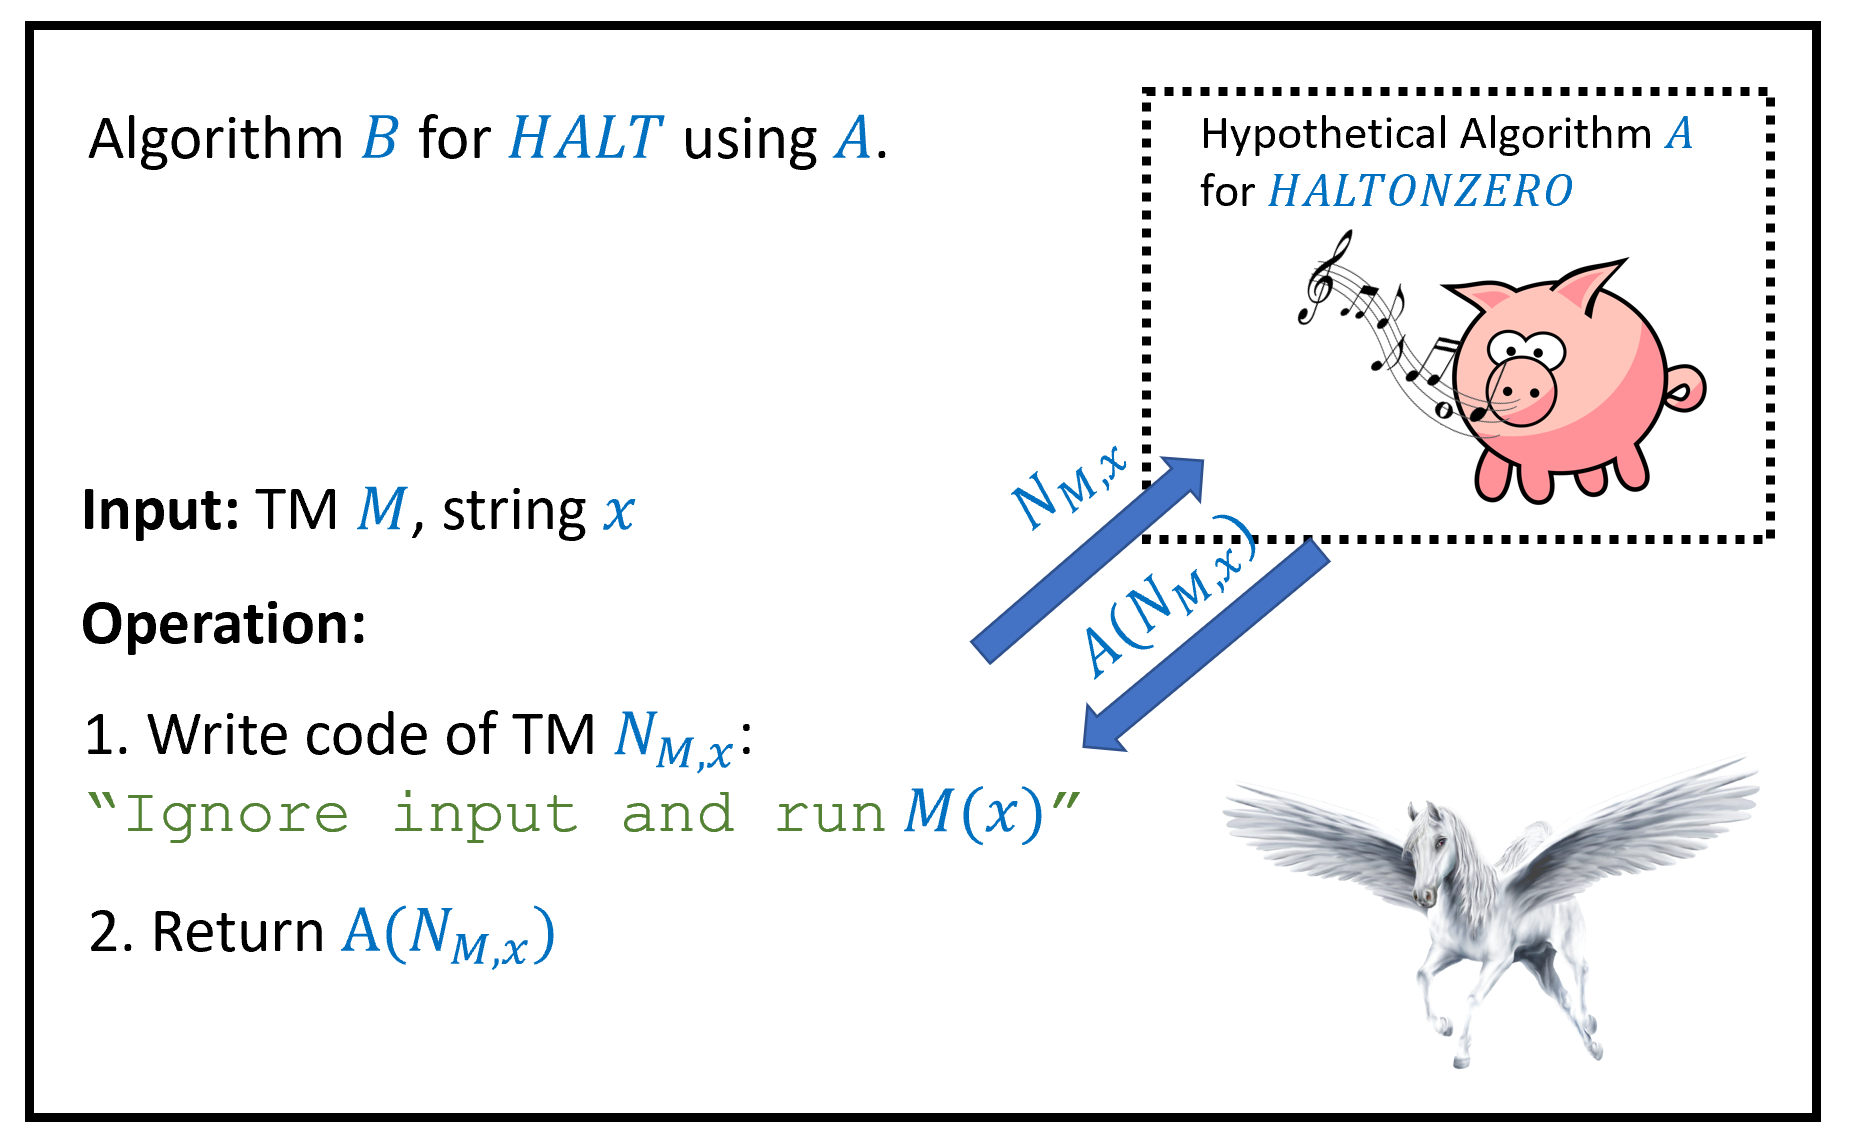
\includegraphics[width=\textwidth, height=0.25\paperheight, keepaspectratio]{../figure/haltonzerored.png}
\caption{To prove \cref{haltonzero-thm}, we show that
\(\ensuremath{\mathit{HALTONZERO}}\) is uncomputable by giving a
\emph{reduction} from the task of computing
\(\ensuremath{\mathit{HALT}}\) to the task of computing
\(\ensuremath{\mathit{HALTONZERO}}\). This shows that if there was a
hypothetical algorithm \(A\) computing
\(\ensuremath{\mathit{HALTONZERO}}\), then there would be an algorithm
\(B\) computing \(\ensuremath{\mathit{HALT}}\), contradicting
\cref{halt-thm}. Since neither \(A\) nor \(B\) actually exists, this is
an example of an implication of the form ``if pigs could whistle then
horses could fly''.}
\label{haltonzerofig}
\end{figure}

\begin{proof}[Proof of \cref{haltonzero-thm}] \label[proof]{The-proof-is-by-reduction}

The proof is by reduction from \(\ensuremath{\mathit{HALT}}\), see
\cref{haltonzerofig}. We will assume, towards the sake of contradiction,
that \(\ensuremath{\mathit{HALTONZERO}}\) is computable by some
algorithm \(A\), and use this hypothetical algorithm \(A\) to construct
an algorithm \(B\) to compute \(\ensuremath{\mathit{HALT}}\), hence
obtaining a contradiction to \cref{halt-thm}. (As discussed in
\cref{defalgsec}, following our ``eat your cake and have it too''
paradigm, we just use the generic name ``algorithm'' rather than
worrying whether we model them as Turing machines, NAND-TM programs,
NAND-RAM, etc.; this makes no difference since all these models are
equivalent to one another.)

Since this is our first proof by reduction from the Halting problem, we
will spell it out in more details than usual. Such a proof by reduction
consists of two steps:

\begin{enumerate}
\def\labelenumi{\arabic{enumi}.}
\item
  \emph{Description of the reduction:} We will describe the operation of
  our algorithm \(B\), and how it makes ``function calls'' to the
  hypothetical algorithm \(A\).
\item
  \emph{Analysis of the reduction:} We will then prove that under the
  hypothesis that Algorithm \(A\) computes
  \(\ensuremath{\mathit{HALTONZERO}}\), Algorithm \(B\) will compute
  \(\ensuremath{\mathit{HALT}}\).
\end{enumerate}

\begin{algorithm}[$HALT$ to $HALTONZERO$ reduction]
\label[algorithm]{halttohaltonzerored} ~ \\ \noindent
\begin{algorithmic}[1]
\INPUT  Turing machine $M$ and string $x$.
\OUTPUT  Turing machine $M'$ such that $M$ halts on $x$ iff $M'$ halts on zero
\PROCEDURE{$N_{M,x}$}{$w$} \COMMENT{ Description of the T.M. $N_{M,x}$}
 \RETURN $EVAL(M,x)$ \COMMENT{ Ignore the \INPUT $w$, evaluate $M$ on $x$.}
\ENDPROCEDURE
\RETURN $N_{M,x}$ \COMMENT{ We do not execute $N_{M,x}$: only \RETURN its description}
\end{algorithmic}
\end{algorithm}

Our Algorithm \(B\) works as follows: on input \(M,x\), it runs
\cref{halttohaltonzerored} to obtain a Turing Machine \(M'\), and then
returns \(A(M')\). The machine \(M'\) ignores its input \(z\) and simply
runs \(M\) on \(x\).

In pseudocode, the program \(N_{M,x}\) will look something like the
following:

\begin{code}
def N(z):
    M = r'.......'
    # a string constant containing desc. of M
    x = r'.......'
    # a string constant containing x
    return eval(M,x)
    # note that we ignore the input z
\end{code}

That is, if we think of \(N_{M,x}\) as a program, then it is a program
that contains \(M\) and \(x\) as ``hardwired constants'', and given any
input \(z\), it simply ignores the input and always returns the result
of evaluating \(M\) on \(x\). The algorithm \(B\) does \emph{not}
actually execute the machine \(N_{M,x}\). \(B\) merely writes down the
description of \(N_{M,x}\) as a string (just as we did above) and feeds
this string as input to \(A\).

The above completes the \emph{description} of the reduction. The
\emph{analysis} is obtained by proving the following claim:

\textbf{Claim:} For every strings \(M,x,z\), the machine \(N_{M,x}\)
constructed by Algorithm \(B\) in Step 1 satisfies that \(N_{M,x}\)
halts on \(z\) if and only if the program described by \(M\) halts on
the input \(x\).

\textbf{Proof of Claim:} Since \(N_{M,x}\) ignores its input and
evaluates \(M\) on \(x\) using the universal Turing machine, it will
halt on \(z\) if and only if \(M\) halts on \(x\).

In particular if we instantiate this claim with the input \(z=0\) to
\(N_{M,x}\), we see that
\(\ensuremath{\mathit{HALTONZERO}}(N_{M,x})=\ensuremath{\mathit{HALT}}(M,x)\).
Thus if the hypothetical algorithm \(A\) satisfies
\(A(M)=\ensuremath{\mathit{HALTONZERO}}(M)\) for every \(M\) then the
algorithm \(B\) we construct satisfies
\(B(M,x)=\ensuremath{\mathit{HALT}}(M,x)\) for every \(M,x\),
contradicting the uncomputability of \(\ensuremath{\mathit{HALT}}\).

\end{proof}

\hypertarget{hardwiringrem}{}
\begin{remark}[The hardwiring technique] \label[remark]{hardwiringrem}

In the proof of \cref{haltonzero-thm} we used the technique of
``hardwiring'' an input \(x\) to a program/machine \(P\). That is,
modifying a program \(P\) that it uses ``hardwired constants'' for some
of all of its input. This technique is quite common in reductions and
elsewhere, and we will often use it again in this course.

\end{remark}

\section{Rice's Theorem and the impossibility of general software
verification}\label{Rices-Theorem-and-the-imp}

The uncomputability of the Halting problem turns out to be a special
case of a much more general phenomenon. Namely, that \emph{we cannot
certify semantic properties of general purpose programs}. ``Semantic
properties'' mean properties of the \emph{function} that the program
computes, as opposed to properties that depend on the particular syntax
used by the program.

An example for a \emph{semantic property} of a program \(P\) is the
property that whenever \(P\) is given an input string with an even
number of \(1\)'s, it outputs \(0\). Another example is the property
that \(P\) will always halt whenever the input ends with a \(1\). In
contrast, the property that a C program contains a comment before every
function declaration is not a semantic property, since it depends on the
actual source code as opposed to the input/output relation.

Checking semantic properties of programs is of great interest, as it
corresponds to checking whether a program conforms to a specification.
Alas it turns out that such properties are in general
\emph{uncomputable}. We have already seen some examples of uncomputable
semantic functions, namely \(\ensuremath{\mathit{HALT}}\) and
\(\ensuremath{\mathit{HALTONZERO}}\), but these are just the ``tip of
the iceberg''. We start by observing one more such example:

\hypertarget{allzero-thm}{}
\begin{theorem}[Computing all zero function] \label[theorem]{allzero-thm}

Let \(\ensuremath{\mathit{ZEROFUNC}}:\{0,1\}^* \rightarrow \{0,1\}\) be
the function such that for every \(M\in \{0,1\}^*\),
\(\ensuremath{\mathit{ZEROFUNC}}(M)=1\) if and only if \(M\) represents
a Turing machine such that \(M\) outputs \(0\) on every input
\(x\in \{0,1\}^*\). Then \(\ensuremath{\mathit{ZEROFUNC}}\) is
uncomputable.

\end{theorem}

\begin{pause} \label[pause]{Despite-the-similarity-in}

Despite the similarity in their names,
\(\ensuremath{\mathit{ZEROFUNC}}\) and
\(\ensuremath{\mathit{HALTONZERO}}\) are two different functions. For
example, if \(M\) is a Turing machine that on input \(x \in \{0,1\}^*\),
halts and outputs the OR of all of \(x\)'s coordinates, then
\(\ensuremath{\mathit{HALTONZERO}}(M)=1\) (since \(M\) does halt on the
input \(0\)) but \(\ensuremath{\mathit{ZEROFUNC}}(M)=0\) (since \(M\)
does not compute the constant zero function).

\end{pause}

\begin{proof}[Proof of \cref{allzero-thm}] \label[proof]{The-proof-is-by-reduction}

The proof is by reduction to \(\ensuremath{\mathit{HALTONZERO}}\).
Suppose, towards the sake of contradiction, that there was an algorithm
\(A\) such that \(A(M)=\ensuremath{\mathit{ZEROFUNC}}(M)\) for every
\(M \in \{0,1\}^*\). Then we will construct an algorithm \(B\) that
solves \(\ensuremath{\mathit{HALTONZERO}}\), contradicting
\cref{haltonzero-thm}.

Given a Turing machine \(N\) (which is the input to
\(\ensuremath{\mathit{HALTONZERO}}\)), our Algorithm \(B\) does the
following:

\begin{enumerate}
\def\labelenumi{\arabic{enumi}.}
\item
  Construct a Turing Machine \(M\) which on input \(x\in\{0,1\}^*\),
  first runs \(N(0)\) and then outputs \(0\).
\item
  Return \(A(M)\).
\end{enumerate}

Now if \(N\) halts on the input \(0\) then the Turing machine \(M\)
computes the constant zero function, and hence under our assumption that
\(A\) computes \(\ensuremath{\mathit{ZEROFUNC}}\), \(A(M)=1\). If \(N\)
does not halt on the input \(0\), then the Turing machine \(M\) will not
halt on any input, and so in particular will \emph{not} compute the
constant zero function. Hence under our assumption that \(A\) computes
\(\ensuremath{\mathit{ZEROFUNC}}\), \(A(M)=0\). We see that in both
cases,
\(\ensuremath{\mathit{ZEROFUNC}}(M)=\ensuremath{\mathit{HALTONZERO}}(N)\)
and hence the value that Algorithm \(B\) returns in step 2 is equal to
\(\ensuremath{\mathit{HALTONZERO}}(N)\) which is what we needed to
prove.

\end{proof}

Another result along similar lines is the following:

\hypertarget{paritythm}{}
\begin{theorem}[Uncomputability of verifying parity] \label[theorem]{paritythm}

The following function is uncomputable \[
\ensuremath{\mathit{COMPUTES}}\text{-}\ensuremath{\mathit{PARITY}}(P) = \begin{cases} 1 & P \text{ computes the parity function } \\ 0 & \text{otherwise} \end{cases}
\]

\end{theorem}

\begin{pause} \label[pause]{We-leave-the-proof-of-cre}

We leave the proof of \cref{paritythm} as an exercise
(\cref{paritythmex}). I strongly encourage you to stop here and try to
solve this exercise.

\end{pause}

\subsection{Rice's Theorem}\label{ricethmsec}

\cref{paritythm} can be generalized far beyond the parity function. In
fact, this generalization rules out verifying any type of semantic
specification on programs. We define a \emph{semantic specification} on
programs to be some property that does not depend on the code of the
program but just on the function that the program computes.

For example, consider the following two C programs

\begin{code}
int First(int k) {
    return 2*k;
}
\end{code}

\begin{code}
int Second(int n) {
    int i = 0;
    int j = 0
    while (j<n) {
        i = i + 2;
        j=  j + 1;
    }
    return i;
}
\end{code}

\texttt{First} and \texttt{Second} are two distinct C programs, but they
compute the same function. A \emph{semantic} property, would be either
\emph{true} for both programs or \emph{false} for both programs, since
it depends on the \emph{function} the programs compute and not on their
code. An example for a semantic property that both \texttt{First} and
\texttt{Second} satisfy is the following: \emph{``The program \(P\)
computes a function \(f\) mapping integers to integers satisfying that
\(f(n) \geq n\) for every input \(n\)''.}

A property is \emph{not semantic} if it depends on the \emph{source
code} rather than the input/output behavior. For example, properties
such as ``the program contains the variable \texttt{k}'' or ``the
program uses the \texttt{while} operation'' are not semantic. Such
properties can be true for one of the programs and false for others.
Formally, we define semantic properties as follows:

\hypertarget{semanticpropdef}{}
\begin{definition}[Semantic properties] \label[definition]{semanticpropdef}

A pair of Turing machines \(M\) and \(M'\) are \emph{functionally
equivalent} if for every \(x\in \{0,1\}^*\), \(M(x)=M'(x)\). (In
particular, \(M(x)=\bot\) iff \(M'(x)=\bot\) for all \(x\).)

A function \(F:\{0,1\}^* \rightarrow \{0,1\}\) is \emph{semantic} if for
every pair of strings \(M,M'\) that represent functionally equivalent
Turing machines, \(F(M)=F(M')\). (Recall that we assume that every
string represents \emph{some} Turing machine, see \cref{TMrepremark})

\end{definition}

There are two trivial examples of semantic functions: the constant one
function and the constant zero function. For example, if \(Z\) is the
constant zero function (i.e., \(Z(M)=0\) for every \(M\)) then clearly
\(F(M)=F(M')\) for every pair of Turing machines \(M\) and \(M'\) that
are functionally equivalent \(M\) and \(M'\). Here is a non-trivial
example

\hypertarget{zerofuncsem}{}
\begin{solvedexercise}[$ZEROFUNC$ is semantic] \label[solvedexercise]{zerofuncsem}

Prove that the function \(\ensuremath{\mathit{ZEROFUNC}}\) is semantic.

\end{solvedexercise}

\begin{solution} \label[solution]{Recall-that-ensuremathmat}

Recall that \(\ensuremath{\mathit{ZEROFUNC}}(M)=1\) if and only if
\(M(x)=0\) for every \(x\in \{0,1\}^*\). If \(M\) and \(M'\) are
functionally equivalent, then for every \(x\), \(M(x)=M'(x)\). Hence
\(\ensuremath{\mathit{ZEROFUNC}}(M)=1\) if and only if
\(\ensuremath{\mathit{ZEROFUNC}}(M')=1\).

\end{solution}

Often the properties of programs that we are most interested in
computing are the \emph{semantic} ones, since we want to understand the
programs' functionality. Unfortunately, Rice's Theorem tells us that
these properties are all uncomputable:

\hypertarget{rice-thm}{}
\begin{theorem}[Rice's Theorem] \label[theorem]{rice-thm}

Let \(F:\{0,1\}^* \rightarrow \{0,1\}\). If \(F\) is semantic and
non-trivial then it is uncomputable.

\end{theorem}

\begin{proofidea} \label[proofidea]{The-idea-behind-the-proof}

The idea behind the proof is to show that every semantic non-trivial
function \(F\) is at least as hard to compute as
\(\ensuremath{\mathit{HALTONZERO}}\). This will conclude the proof since
by \cref{haltonzero-thm}, \(\ensuremath{\mathit{HALTONZERO}}\) is
uncomputable. If a function \(F\) is non trivial then there are two
machines \(M_0\) and \(M_1\) such that \(F(M_0)=0\) and \(F(M_1)=1\).
So, the goal would be to take a machine \(N\) and find a way to map it
into a machine \(M=R(N)\), such that \textbf{(i)} if \(N\) halts on zero
then \(M\) is functionally equivalent to \(M_1\) and \textbf{(ii)} if
\(N\) does \emph{not} halt on zero then \(M\) is functionally equivalent
\(M_0\).

Because \(F\) is semantic, if we achieved this, then we would be
guaranteed that \(\ensuremath{\mathit{HALTONZERO}}(N) = F(R(N))\), and
hence would show that if \(F\) was computable, then
\(\ensuremath{\mathit{HALTONZERO}}\) would be computable as well,
contradicting \cref{haltonzero-thm}.

\end{proofidea}

\begin{proof}[Proof of \cref{rice-thm}] \label[proof]{We-will-not-give-the-proo}

We will not give the proof in full formality, but rather illustrate the
proof idea by restricting our attention to a particular semantic
function \(F\). However, the same techniques generalize to all possible
semantic functions. Define
\(\ensuremath{\mathit{MONOTONE}}:\{0,1\}^* \rightarrow \{0,1\}\) as
follows: \(\ensuremath{\mathit{MONOTONE}}(M)=1\) if there does not exist
\(n\in \N\) and two inputs \(x,x' \in \{0,1\}^n\) such that for every
\(i\in [n]\) \(x_i \leq x'_i\) but \(M(x)\) outputs \(1\) and
\(M(x')=0\). That is, \(\ensuremath{\mathit{MONOTONE}}(M)=1\) if it's
not possible to find an input \(x\) such that flipping some bits of
\(x\) from \(0\) to \(1\) will change \(M\)'s output in the other
direction from \(1\) to \(0\). We will prove that
\(\ensuremath{\mathit{MONOTONE}}\) is uncomputable, but the proof will
easily generalize to any semantic function.

We start by noting that \(\ensuremath{\mathit{MONOTONE}}\) is neither
the constant zero nor the constant one function:

\begin{itemize}
\item
  The machine \(\ensuremath{\mathit{INF}}\) that simply goes into an
  infinite loop on every input satisfies
  \(\ensuremath{\mathit{MONOTONE}}(\ensuremath{\mathit{INF}})=1\), since
  \(\ensuremath{\mathit{INF}}\) is not defined \emph{anywhere} and so in
  particular there are no two inputs \(x,x'\) where \(x_i \leq x'_i\)
  for every \(i\) but \(\ensuremath{\mathit{INF}}(x)=0\) and
  \(\ensuremath{\mathit{INF}}(x')=1\).
\item
  The machine \(\ensuremath{\mathit{PAR}}\) that computes the XOR or
  parity of its input, is not monotone (e.g.,
  \(\ensuremath{\mathit{PAR}}(1,1,0,0,\ldots,0)=0\) but
  \(\ensuremath{\mathit{PAR}}(1,0,0,\ldots,0)=0\)) and hence
  \(\ensuremath{\mathit{MONOTONE}}(\ensuremath{\mathit{PAR}})=0\).
\end{itemize}

(Note that \(\ensuremath{\mathit{INF}}\) and
\(\ensuremath{\mathit{PAR}}\) are \emph{machines} and not
\emph{functions}.)

We will now give a reduction from \(\ensuremath{\mathit{HALTONZERO}}\)
to \(\ensuremath{\mathit{MONOTONE}}\). That is, we assume towards a
contradiction that there exists an algorithm \(A\) that computes
\(\ensuremath{\mathit{MONOTONE}}\) and we will build an algorithm \(B\)
that computes \(\ensuremath{\mathit{HALTONZERO}}\). Our algorithm \(B\)
will work as follows:

\begin{quote} \label[quote]{Algorithm-BInput-String-N}

\textbf{Algorithm \(B\):}

\textbf{Input:} String \(N\) describing a Turing machine. (\emph{Goal:}
Compute \(\ensuremath{\mathit{HALTONZERO}}(N)\))

\textbf{Assumption:} Access to Algorithm \(A\) to compute
\(\ensuremath{\mathit{MONOTONE}}\).

\textbf{Operation:}

\begin{enumerate}
\def\labelenumi{\arabic{enumi}.}
\item
  Construct the following machine \(M\): ``On input \(z\in \{0,1\}^*\)
  do: \textbf{(a)} Run \(N(0)\), \textbf{(b)} Return
  \(\ensuremath{\mathit{PAR}}(z)\)''.
\item
  Return \(1-A(M)\).
\end{enumerate}

\end{quote}

To complete the proof we need to show that \(B\) outputs the correct
answer, under our assumption that \(A\) computes
\(\ensuremath{\mathit{MONOTONE}}\). In other words, we need to show that
\(\ensuremath{\mathit{HALTONZERO}}(N)=1-MONOTONE(M)\). Suppose that
\(N\) does \emph{not} halt on zero. In this case the program \(M\)
constructed by Algorithm \(B\) enters into an infinite loop in step
\textbf{(a)} and will never reach step \textbf{(b)}. Hence in this case
\(N\) is functionally equivalent to \(\ensuremath{\mathit{INF}}\). (The
machine \(N\) is not the same machine as \(\ensuremath{\mathit{INF}}\):
its description or \emph{code} is different. But it does have the same
input/output behavior (in this case) of never halting on any input.
Also, while the program \(M\) will go into an infinite loop on every
input, Algorithm \(B\) never actually runs \(M\): it only produces its
code and feeds it to \(A\). Hence Algorithm \(B\) will \emph{not} enter
into an infinite loop even in this case.) Thus in this case,
\(\ensuremath{\mathit{MONOTONE}}(N)=\ensuremath{\mathit{MONOTONE}}(\ensuremath{\mathit{INF}})=1\).

If \(N\) \emph{does} halt on zero, then step \textbf{(a)} in \(M\) will
eventually conclude and \(M\)'s output will be determined by step
\textbf{(b)}, where it simply outputs the parity of its input. Hence in
this case, \(M\) computes the non-monotone parity function (i.e., is
functionally equivalent to \(\ensuremath{\mathit{PAR}}\)), and so we get
that
\(\ensuremath{\mathit{MONOTONE}}(M)=\ensuremath{\mathit{MONOTONE}}(\ensuremath{\mathit{PAR}})=0\).
In both cases, \(\ensuremath{\mathit{MONOTONE}}(M)=1-HALTONZERO(N)\),
which is what we wanted to prove.

An examination of this proof shows that we did not use anything about
\(\ensuremath{\mathit{MONOTONE}}\) beyond the fact that it is semantic
and non-trivial. For every semantic non-trivial \(F\), we can use the
same proof, replacing \(\ensuremath{\mathit{PAR}}\) and
\(\ensuremath{\mathit{INF}}\) with two machines \(M_0\) and \(M_1\) such
that \(F(M_0)=0\) and \(F(M_1)=1\). Such machines must exist if \(F\) is
non trivial.

\end{proof}

\hypertarget{syntacticcomputablefunctions}{}
\begin{remark}[Semantic is not the same as uncomputable] \label[remark]{syntacticcomputablefunctions}

Rice's Theorem is so powerful and such a popular way of proving
uncomputability that people sometimes get confused and think that it is
the \emph{only} way to prove uncomputability. In particular, a common
misconception is that if a function \(F\) is \emph{not} semantic then it
is \emph{computable}. This is not at all the case.

For example, consider the following function
\(\ensuremath{\mathit{HALTNOYALE}}:\{0,1\}^* \rightarrow \{0,1\}\). This
is a function that on input a string that represents a NAND-TM program
\(P\), outputs \(1\) if and only if both \textbf{(i)} \(P\) halts on the
input \(0\), and \textbf{(ii)} the program \(P\) does not contain a
variable with the identifier \texttt{Yale}. The function
\(\ensuremath{\mathit{HALTNOYALE}}\) is clearly not semantic, as it will
output two different values when given as input one of the following two
functionally equivalent programs:

\begin{code}
Yale[0] = NAND(X[0],X[0])
Y[0] = NAND(X[0],Yale[0])
\end{code}

and

\begin{code}
Harvard[0] = NAND(X[0],X[0])
Y[0] = NAND(X[0],Harvard[0])
\end{code}

However, \(\ensuremath{\mathit{HALTNOYALE}}\) is uncomputable since
every program \(P\) can be transformed into an equivalent (and in fact
improved \texttt{:)}) program \(P'\) that does not contain the variable
\texttt{Yale}. Hence if we could compute
\(\ensuremath{\mathit{HALTONYALE}}\) then determine halting on zero for
NAND-TM programs (and hence for Turing machines as well).

Moreover, as we will see in \cref{godelchap}, there are uncomputable
functions whose inputs are not programs, and hence for which the
adjective ``semantic'' is not applicable.

Properties such as ``the program contains the variable \texttt{Yale}''
are sometimes known as \emph{syntactic} properties. The terms
``semantic'' and ``syntactic'' are used beyond the realm of programming
languages: a famous example of a syntactically correct but semantically
meaningless sentence in English is Chomsky's
\href{https://goo.gl/4gXoiV}{``Colorless green ideas sleep furiously.''}
However, formally defining ``syntactic properties'' is rather subtle and
we will not use this terminology in this book, sticking to the terms
``semantic'' and ``non semantic'' only.

\end{remark}

\subsection{Halting and Rice's Theorem for other Turing-complete
models}\label{Halting-and-Rices-Theorem}

As we saw before, many natural computational models turn out to be
\emph{equivalent} to one another, in the sense that we can transform a
``program'' of one model (such as a \(\lambda\) expression, or a
game-of-life configurations) into another model (such as a NAND-TM
program). This equivalence implies that we can translate the
uncomputability of the Halting problem for NAND-TM programs into
uncomputability for Halting in other models. For example:

\hypertarget{halt-tm}{}
\begin{theorem}[NAND-TM Machine Halting] \label[theorem]{halt-tm}

Let \(\ensuremath{\mathit{NANDTMHALT}}:\{0,1\}^* \rightarrow \{0,1\}\)
be the function that on input strings \(P\in\{0,1\}^*\) and
\(x\in \{0,1\}^*\) outputs \(1\) if the NAND-TM program described by
\(P\) halts on the input \(x\) and outputs \(0\) otherwise. Then
\(\ensuremath{\mathit{NANDTMHALT}}\) is uncomputable.

\end{theorem}

\begin{pause} \label[pause]{Once-again-this-is-a-good}

Once again, this is a good point for you to stop and try to prove the
result yourself before reading the proof below.

\end{pause}

\begin{proof} \label[proof]{We-have-seen-in-crefTM-eq}

We have seen in \cref{TM-equiv-thm} that for every Turing machine \(M\),
there is an equivalent NAND-TM program \(P_M\) such that for every
\(x\), \(P_M(x)=M(x)\). In particular this means that
\(\ensuremath{\mathit{HALT}}(M)= \ensuremath{\mathit{NANDTMHALT}}(P_M)\).

The transformation \(M \mapsto P_M\) that is obtained from the proof of
\cref{TM-equiv-thm} is \emph{constructive}. That is, the proof yields a
way to \emph{compute} the map \(M \mapsto P_M\). This means that this
proof yields a \emph{reduction} from task of computing
\(\ensuremath{\mathit{HALT}}\) to the task of computing
\(\ensuremath{\mathit{NANDTMHALT}}\), which means that since
\(\ensuremath{\mathit{HALT}}\) is uncomputable, neither is
\(\ensuremath{\mathit{NANDTMHALT}}\).

\end{proof}

The same proof carries over to other computational models such as the
\emph{\(\lambda\) calculus}, \emph{two dimensional} (or even
one-dimensional) \emph{automata} etc. Hence for example, there is no
algorithm to decide if a \(\lambda\) expression evaluates the identity
function, and no algorithm to decide whether an initial configuration of
the game of life will result in eventually coloring the cell \((0,0)\)
black or not.

Indeed, we can generalize Rice's Theorem to all these models. For
example, if \(F:\{0,1\}^* \rightarrow \{0,1\}\) is a non-trivial
function such that \(F(P)=F(P')\) for every functionally equivalent
NAND-TM programs \(P,P'\) then \(F\) is uncomputable, and the same holds
for NAND-RAM programs, \(\lambda\)-expressions, and all other Turing
complete models (as defined in \cref{turingcompletedef}), see also
\cref{ricegeneralex}.

\subsection{Is software verification doomed?
(discussion)}\label{Is-software-verification-}

Programs are increasingly being used for mission critical purposes,
whether it's running our banking system, flying planes, or monitoring
nuclear reactors. If we can't even give a certification algorithm that a
program correctly computes the parity function, how can we ever be
assured that a program does what it is supposed to do? The key insight
is that while it is impossible to certify that a \emph{general} program
conforms with a specification, it is possible to write a program in the
first place in a way that will make it easier to certify. As a trivial
example, if you write a program without loops, then you can certify that
it halts. Also, while it might not be possible to certify that an
\emph{arbitrary} program computes the parity function, it is quite
possible to write a particular program \(P\) for which we can
mathematically \emph{prove} that \(P\) computes the parity. In fact,
writing programs or algorithms and providing proofs for their
correctness is what we do all the time in algorithms research.

The field of \emph{software verification} is concerned with verifying
that given programs satisfy certain conditions. These conditions can be
that the program computes a certain function, that it never writes into
a dangerous memory location, that is respects certain invariants, and
others. While the general tasks of verifying this may be uncomputable,
researchers have managed to do so for many interesting cases, especially
if the program is written in the first place in a formalism or
programming language that makes verification easier. That said,
verification, especially of large and complex programs, remains a highly
challenging task in practice as well, and the number of programs that
have been formally proven correct is still quite small. Moreover, even
phrasing the right theorem to prove (i.e., the specification) if often a
highly non-trivial endeavor.


\begin{figure}
\centering
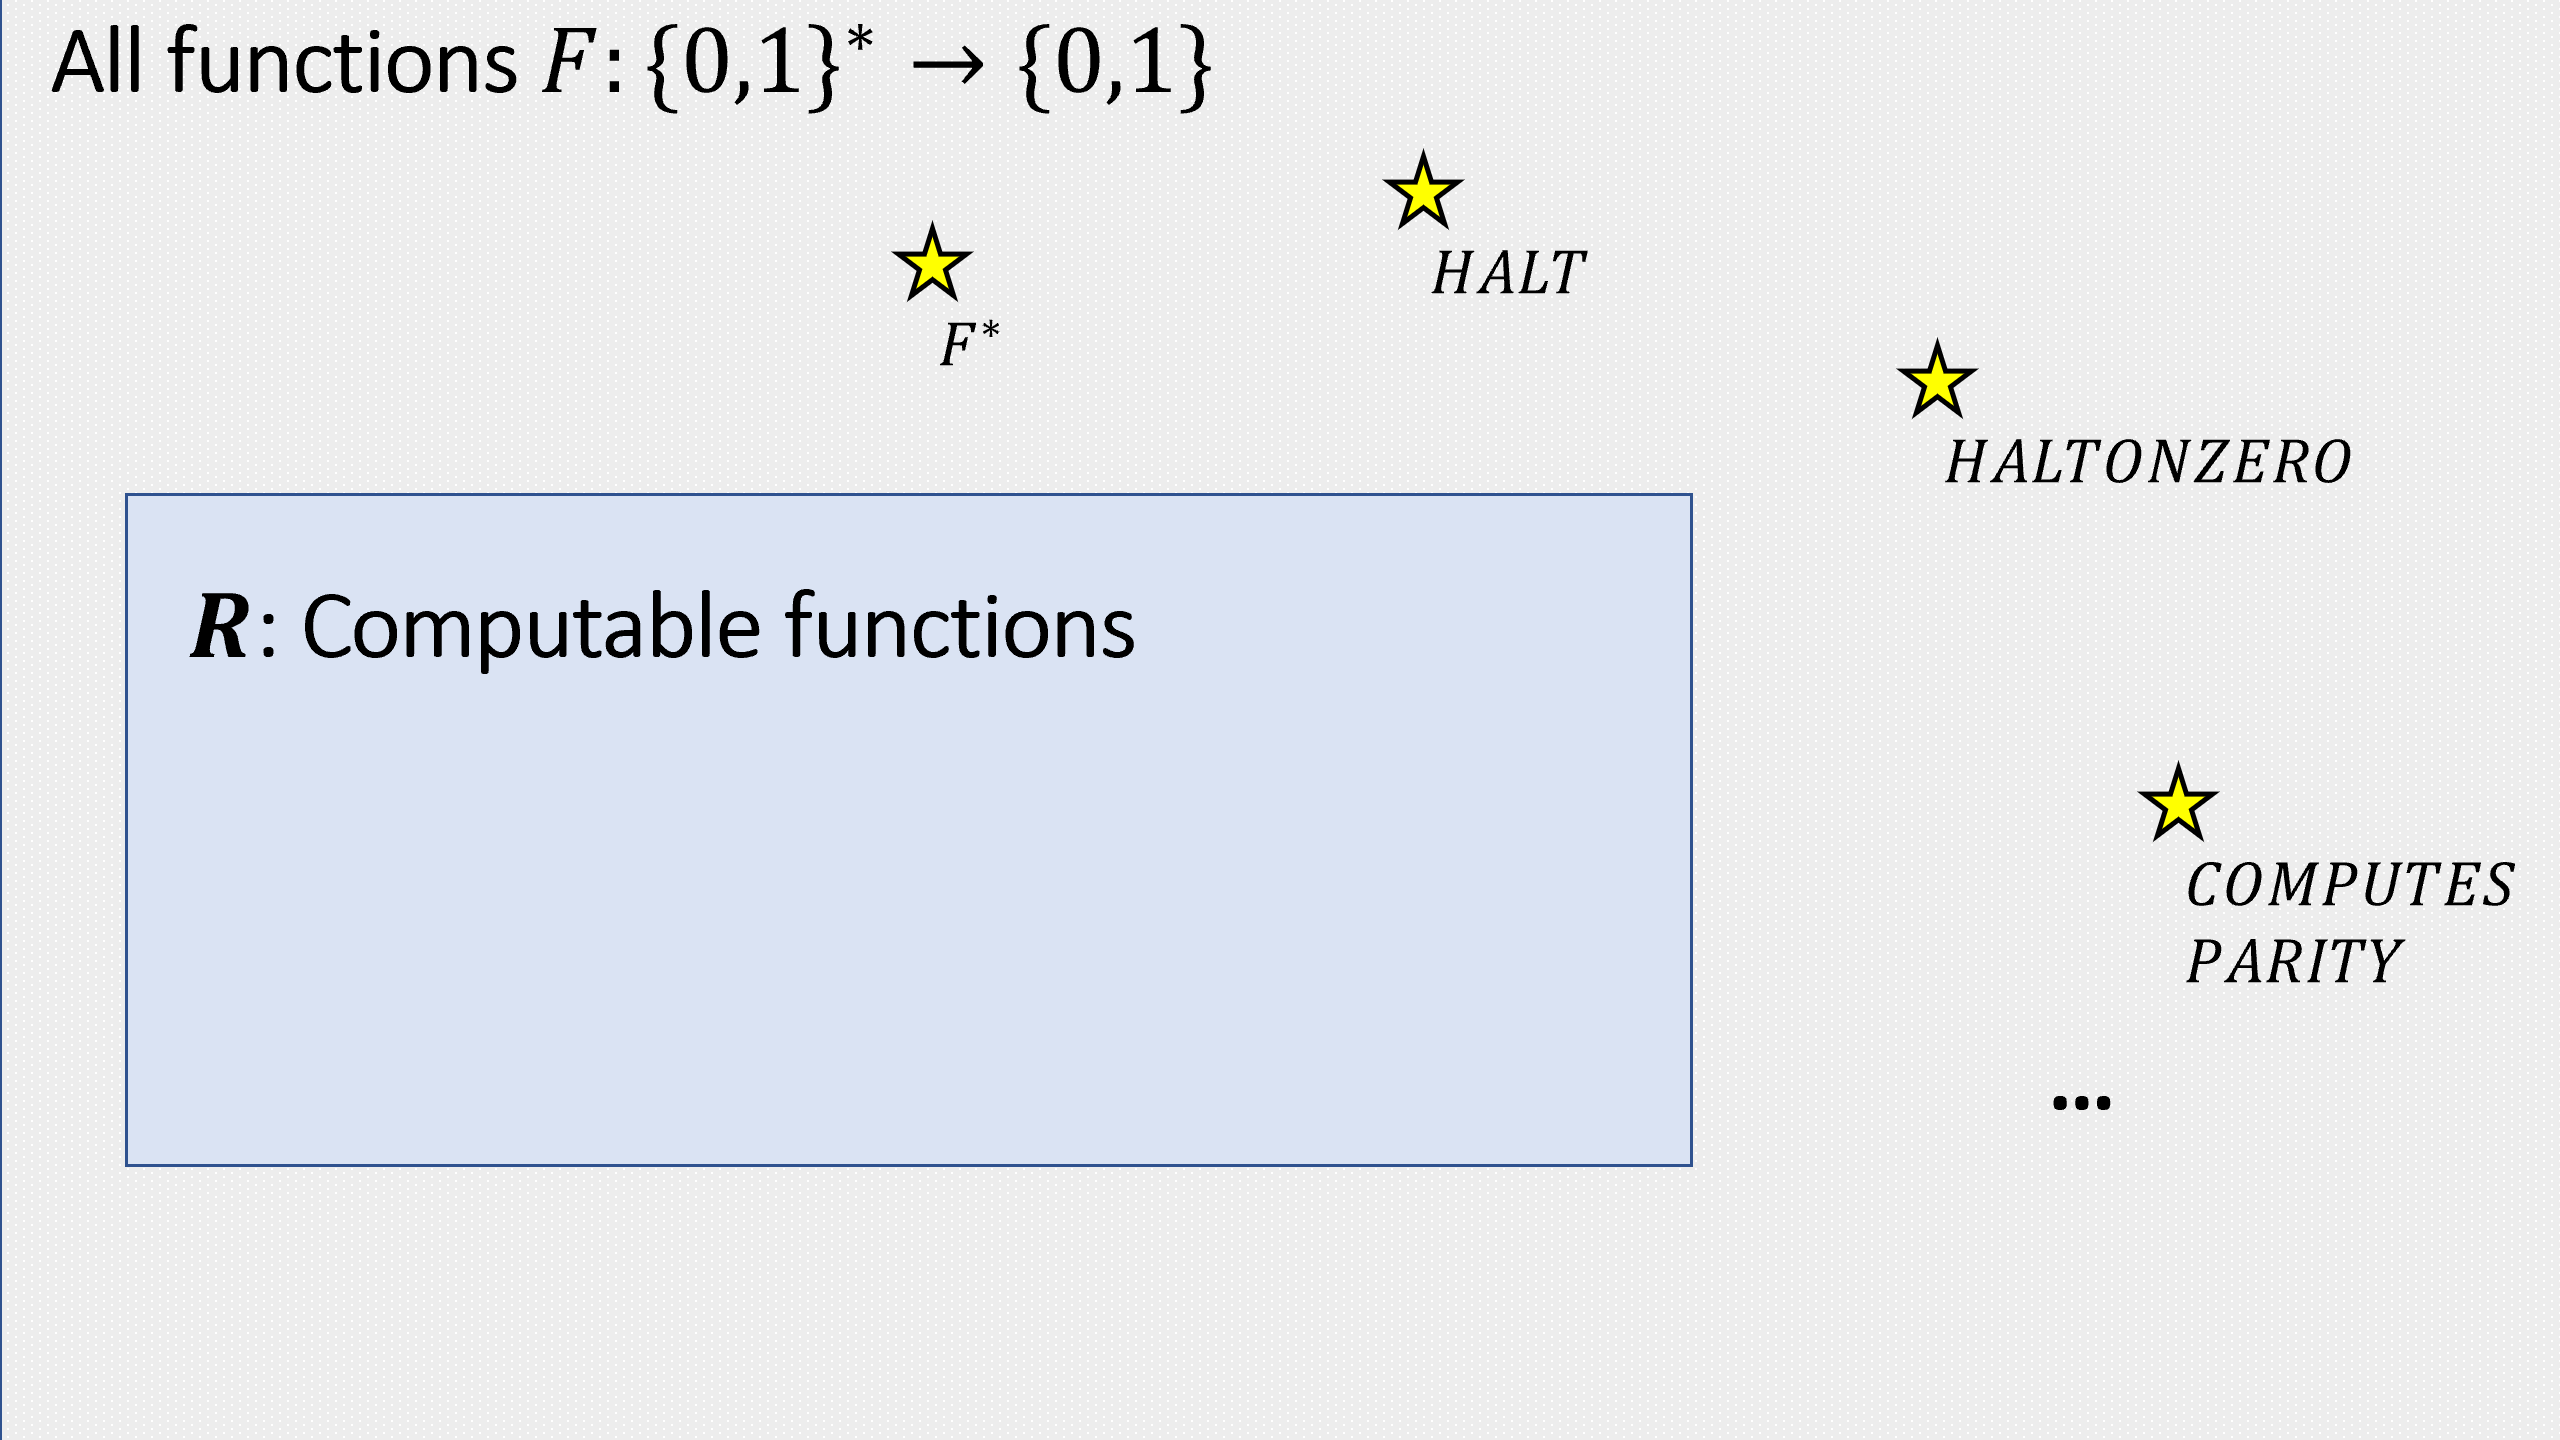
\includegraphics[width=\textwidth, height=0.25\paperheight, keepaspectratio]{../figure/inclusion_noncomputable.png}
\caption{The set \(\mathbf{R}\) of computable Boolean functions
(\cref{classRdef}) is a proper subset of the set of all functions
mapping \(\{0,1\}^*\) to \(\{0,1\}\). In this chapter we saw a few
examples of elements in the latter set that are not in the former.}
\label{inclusionuncomputablefig}
\end{figure}

\begin{recap} \label[recap]{There-is-a-universal-Turi}

\begin{itemize}
\item
  There is a \emph{universal} Turing machine (or NAND-TM program) \(U\)
  such that on input a description of a Turing machine \(M\) and some
  input \(x\), \(U(M,x)\) halts and outputs \(M(x)\) if (and only if)
  \(M\) halts on input \(x\). Unlike in the case of finite computation
  (i.e., NAND-CIRC programs / circuits), the input to the program \(U\)
  can be a machine \(M\) that has more states than \(U\) itself.
\item
  Unlike the finite case, there are actually functions that are
  \emph{inherently uncomputable} in the sense that they cannot be
  computed by \emph{any} Turing machine.
\item
  These include not only some ``degenerate'' or ``esoteric'' functions
  but also functions that people have deeply care about and conjectured
  that could be computed.
\item
  If the Church-Turing thesis holds then a function \(F\) that is
  uncomputable according to our definition cannot be computed by any
  means in our physical world.
\end{itemize}

\end{recap}

\section{Exercises}\label{Exercises}

\hypertarget{NANDRAMHalt}{}
\begin{exercise}[NAND-RAM Halt] \label[exercise]{NANDRAMHalt}

Let \(\ensuremath{\mathit{NANDRAMHALT}}:\{0,1\}^* \rightarrow \{0,1\}\)
be the function such that on input \((P,x)\) where \(P\) represents a
NAND-RAM program, \(\ensuremath{\mathit{NANDRAMHALT}}(P,x)=1\) iff \(P\)
halts on the input \(x\). Prove that
\(\ensuremath{\mathit{NANDRAMHALT}}\) is uncomputable.

\end{exercise}

\hypertarget{timedhalt}{}
\begin{exercise}[Timed halting] \label[exercise]{timedhalt}

Let \(\ensuremath{\mathit{TIMEDHALT}}:\{0,1\}^* \rightarrow \{0,1\}\) be
the function that on input (a string representing) a triple \((M,x,T)\),
\(\ensuremath{\mathit{TIMEDHALT}}(M,x,T)=1\) iff the Turing machine
\(M\), on input \(x\), halts within at most \(T\) steps (where a
\emph{step} is defined as one sequence of reading a symbol from the
tape, updating the state, writing a new symbol and (potentially) moving
the head).

Prove that \(\ensuremath{\mathit{TIMEDHALT}}\) is \emph{computable}.

\end{exercise}

\hypertarget{spacehalting}{}
\begin{exercise}[Space halting (challenging)] \label[exercise]{spacehalting}

Let \(\ensuremath{\mathit{SPACEHALT}}:\{0,1\}^* \rightarrow \{0,1\}\) be
the function that on input (a string representing) a triple \((M,x,T)\),
\(\ensuremath{\mathit{SPACEHALT}}(M,x,T)=1\) iff the Turing machine
\(M\), on input \(x\), halts before its head reached the \(T\)-th
location of its tape. (We don't care how many steps \(M\) makes, as long
as the head stays inside locations \(\{0,\ldots,T-1\}\).)

Prove that \(\ensuremath{\mathit{SPACEHALT}}\) is \emph{computable}. See
footnote for hint\footnote{A machine with alphabet \(\Sigma\) can have
  at most \(|\Sigma|^T\) choices for the contents of the first \(T\)
  locations of its tape. What happens if the machine repeats a
  previously seen configuration, in the sense that the tape contents,
  the head location, and the current state, are all identical to what
  they were in some previous state of the execution?}

\end{exercise}

\hypertarget{necessarilyuncomputableex}{}
\begin{exercise}[Computable compositions] \label[exercise]{necessarilyuncomputableex}

Suppose that \(F:\{0,1\}^* \rightarrow \{0,1\}\) and
\(G:\{0,1\}^* \rightarrow \{0,1\}\) are computable functions. For each
one of the following functions \(H\), either prove that \(H\) is
\emph{necessarily computable} or give an example of a pair \(F\) and
\(G\) of computable functions such that \(H\) will not be computable.
Prove your assertions.

\begin{enumerate}
\def\labelenumi{\arabic{enumi}.}
\item
  \(H(x)=1\) iff \(F(x)=1\) OR \(G(x)=1\).
\item
  \(H(x)=1\) iff there exist two nonempty strings \(u,v \in \{0,1\}^*\)
  such that \(x=uv\) (i.e., \(x\) is the concatenation of \(u\) and
  \(v\)), \(F(u)=1\) and \(G(v)=1\).
\item
  \(H(x)=1\) iff there exist a list \(u_0,\ldots,u_{t-1}\) of non empty
  strings such that strings\(F(u_i)=1\) for every \(i\in [t]\) and
  \(x=u_0u_1\cdots u_{t-1}\).
\item
  \(H(x)=1\) iff \(x\) is a valid string representation of a NAND++
  program \(P\) such that for every \(z\in \{0,1\}^*\), on input \(z\)
  the program \(P\) outputs \(F(z)\).
\item
  \(H(x)=1\) iff \(x\) is a valid string representation of a NAND++
  program \(P\) such that on input \(x\) the program \(P\) outputs
  \(F(x)\).
\item
  \(H(x)=1\) iff \(x\) is a valid string representation of a NAND++
  program \(P\) such that on input \(x\), \(P\) outputs \(F(x)\) after
  executing at most \(100\cdot |x|^2\) lines.
\end{enumerate}

\end{exercise}

\hypertarget{finiteuncompex}{}
\begin{exercise} \label[exercise]{finiteuncompex}

Prove that the following function
\(\ensuremath{\mathit{FINITE}}:\{0,1\}^* \rightarrow \{0,1\}\) is
uncomputable. On input \(P\in \{0,1\}^*\), we define
\(\ensuremath{\mathit{FINITE}}(P)=1\) if and only if \(P\) is a string
that represents a NAND++ program such that there only a finite number of
inputs \(x\in \{0,1\}^*\) s.t. \(P(x)=1\).\footnote{Hint: You can use
  Rice's Theorem.}

\end{exercise}

\hypertarget{paritythmex}{}
\begin{exercise}[Computing parity] \label[exercise]{paritythmex}

Prove \cref{paritythm} without using Rice's Theorem.

\end{exercise}

\hypertarget{TMequivex}{}
\begin{exercise}[TM Equivalence] \label[exercise]{TMequivex}

Let \(\ensuremath{\mathit{EQ}}:\{0,1\}^* :\rightarrow \{0,1\}\) be the
function defined as follows: given a string representing a pair
\((M,M')\) of Turing machines, \(\ensuremath{\mathit{EQ}}(M,M')=1\) iff
\(M\) and \(M'\) are functionally equivalent as per
\cref{semanticpropdef}. Prove that \(\ensuremath{\mathit{EQ}}\) is
uncomputable.

Note that you \emph{cannot} use Rice's Theorem directly, as this theorem
only deals with functions that take a single Turing machine as input,
and \(\ensuremath{\mathit{EQ}}\) takes two machines.

\end{exercise}

\hypertarget{salil-ex}{}
\begin{exercise} \label[exercise]{salil-ex}

For each of the following two functions, say whether it is computable or
not:

\begin{enumerate}
\def\labelenumi{\arabic{enumi}.}
\item
  Given a NAND-TM program \(P\), an input \(x\), and a number \(k\),
  when we run \(P\) on \(x\), does the index variable \texttt{i} ever
  reach \(k\)?
\item
  Given a NAND-TM program \(P\), an input \(x\), and a number \(k\),
  when we run \(P\) on \(x\), does \(P\) ever write to an array at index
  \(k\)?
\end{enumerate}

\end{exercise}

\hypertarget{ricetmnandram}{}
\begin{exercise} \label[exercise]{ricetmnandram}

Let \(F:\{0,1\}^* \rightarrow \{0,1\}\) be the function that is defined
as follows. On input a string \(P\) that represents a NAND-RAM program
and a String \(M\) that represents a Turing machine, \(F(P,M)=1\) if and
only if there exists some input \(x\) such \(P\) halts on \(x\) but
\(M\) does not halt on \(x\). Prove that \(F\) is uncomputable. See
footnote for hint.\footnote{\emph{Hint:} While it cannot be applied
  directly, with a little ``massaging'' you can prove this using Rice's
  Theorem.}

\end{exercise}

\hypertarget{recursiveenumerableex}{}
\begin{exercise}[Recursively enumerable] \label[exercise]{recursiveenumerableex}

Define a function \(F:\{0,1\}^* :\rightarrow \{0,1\}\) to be
\emph{recursively enumerable} if there exists a Turing machine \(M\)
such that such that for every \(x\in \{0,1\}^*\), if \(F(x)=1\) then
\(M(x)=1\), and if \(F(x)=0\) then \(M(x)=\bot\). (i.e., if \(F(x)=0\)
then \(M\) does not halt on \(x\).)

\begin{enumerate}
\def\labelenumi{\arabic{enumi}.}
\item
  Prove that every computable \(F\) is also recursively enumerable.
\item
  Prove that there exists \(F\) that is not computable but is
  recursively enumerable. See footnote for hint.\footnote{\(\ensuremath{\mathit{HALT}}\)
    has this property.}
\item
  Prove that there exists a function \(F:\{0,1\}^* \rightarrow \{0,1\}\)
  such that \(F\) is not recursively enumerable. See footnote for
  hint.\footnote{You can either use the diagonalization method to prove
    this directly or show that the set of all recursively enumerable
    functions is \emph{countable}.}
\item
  Prove that there exists a function \(F:\{0,1\}^* \rightarrow \{0,1\}\)
  such that \(F\) is recursively enumerable but the function
  \(\overline{F}\) defined as \(\overline{F}(x)=1-F(x)\) is \emph{not}
  recursively enumerable. See footnote for hint.\footnote{\(\ensuremath{\mathit{HALT}}\)
    has this property: show that if both \(\ensuremath{\mathit{HALT}}\)
    and \(\overline{HALT}\) were recursively enumerable then
    \(\ensuremath{\mathit{HALT}}\) would be in fact computable.}
\end{enumerate}

\end{exercise}

\hypertarget{ricestandardex}{}
\begin{exercise}[Rice's Theorem: standard form] \label[exercise]{ricestandardex}

In this exercise we will prove Rice's Theorem in the form that it is
typically stated in the literature.

For a Turing machine \(M\), define \(L(M) \subseteq \{0,1\}^*\) to be
the set of all \(x\in \{0,1\}^*\) such that \(M\) halts on the input
\(x\) and outputs \(1\). (The set \(L(M)\) is known in the literature as
the \emph{language recognized by \(M\)}. Note that \(M\) might either
output a value other than \(1\) or not halt at all on inputs
\(x\not\in L(M)\). )

\begin{enumerate}
\def\labelenumi{\arabic{enumi}.}
\item
  Prove that for every Turing Machine \(M\), if we define
  \(F_M:\{0,1\}^* \rightarrow \{0,1\}\) to be the function such that
  \(F_M(x)=1\) iff \(x\in L(M)\) then \(F_M\) is \emph{recursively
  enumerable} as defined in \cref{recursiveenumerableex}.
\item
  Use \cref{rice-thm} to prove that for every
  \(G:\{0,1\}^* \rightarrow \{0,1\}\), if \textbf{(a)} \(G\) is neither
  the constant zero nor the constant one function, and \textbf{(b)} for
  every \(M,M'\) such that \(L(M)=L(M')\), \(G(M)=G(M')\), then \(G\) is
  uncomputable. See footnote for hint.\footnote{Show that any \(G\)
    satisfying \textbf{(b)} must be semantic.}
\end{enumerate}

\end{exercise}

\hypertarget{ricegeneralex}{}
\begin{exercise}[Rice's Theorem for general Turing-equivalent models (optional)] \label[exercise]{ricegeneralex}

Let \(\mathcal{F}\) be the set of all partial functions from
\(\{0,1\}^*\) to \(\{0,1\}\) and
\(\mathcal{M}:\{0,1\}^* \rightarrow \mathcal{F}\) be a Turing-equivalent
model as defined in \cref{turingcompletedef}. We define a function
\(F:\{0,1\}^* \rightarrow \{0,1\}\) to be
\emph{\(\mathcal{M}\)-semantic} if there exists some
\(\mathcal{G}:\mathcal{F} \rightarrow \{0,1\}\) such that
\(F(P) = \mathcal{G}(\mathcal{M}(P))\) for every \(P\in \{0,1\}^*\).

Prove that for every \(\mathcal{M}\)-semantic
\(F:\{0,1\}^* \rightarrow \{0,1\}\) that is neither the constant one nor
the constant zero function, \(F\) is uncomputable.

\end{exercise}

\section{Bibliographical notes}\label{uncomputablebibnotes}

The cartoon of the Halting problem in \cref{universalchapoverviewfig}
and taken from
\href{https://www.coopertoons.com/education/haltingproblem/haltingproblem.html/}{Charles
Cooper's website}.

Section 7.2 in \cite{MooreMertens11} gives a highly recommended overview
of uncomputability. Gödel, Escher, Bach \cite{hofstadter1999} is a
classic popular science book that touches on uncomputability, and
unprovability, and specifically Gödel's Theorem that we will see in
\cref{godelchap}. See also the recent book by Holt \cite{Holt2018}.

The history of the definition of a function is intertwined with the
development of mathematics as a field. For many years, a function was
identified (as per Euler's quote above) with the means to calculate the
output from the input. In the 1800's, with the invention of the Fourier
series and with the systematic study of continuity and
differentiability, people have started looking at more general kinds of
functions, but the modern definition of a function as an arbitrary
mapping was not yet universally accepted. For example, in 1899 Poincare
wrote \emph{``we have seen a mass of bizarre functions which appear to
be forced to resemble as little as possible honest functions which serve
some purpose. \ldots{} they are invented on purpose to show that our
ancestor's reasoning was at fault, and we shall never get anything more
than that out of them''.} Some of this fascinating history is discussed
in \cite{grabiner1983gave, Kleiner91, Lutzen2002, grabiner2005the , , }.

The existence of a universal Turing machine, and the uncomputability of
\(\ensuremath{\mathit{HALT}}\) was first shown by Turing in his seminal
paper \cite{Turing37}, though closely related results were shown by
Church a year before. These works built on Gödel's 1931
\emph{incompleteness theorem} that we will discuss in \cref{godelchap}.

Some universal Turing Machines with a small alphabet and number of
states are given in \cite{rogozhin1996small}, including a single-tape
universal Turing machine with the binary alphabet and with less than
\(25\) states; see also the survey \cite{woods2009complexity}. Adam
Yedidia has written
\href{https://github.com/adamyedidia/parsimony}{software} to help in
producing Turing machines with a small number of states. This is related
to the recreational pastime of
\href{https://codegolf.stackexchange.com/}{``Code Golfing''} which is
about solving a certain computational task using the as short as
possible program.

The diagonalization argument used to prove uncomputability of \(F^*\) is
derived from Cantor's argument for the uncountability of the reals
discussed in \cref{chaprepres}.

Christopher Strachey was an English computer scientist and the inventor
of the CPL programming language. He was also an early artificial
intelligence visionary, programming a computer to play Checkers and even
write love letters in the early 1950's, see
\href{https://www.newyorker.com/tech/elements/christopher-stracheys-nineteen-fifties-love-machine}{this
New Yorker article} and
\href{http://www.alpha60.de/art/love_letters/}{this website}.

Rice's Theorem was proven in \cite{rice1953classes}. It is typically
stated in a form somewhat different than what we used, see
\cref{ricesstandardex}.

We do not discuss in the chapter the concept of \emph{recursively
enumerable} languages, but it is covered briefly in
\cref{recursiveenumerableex}. As usual, we use function, as opposto
language, notation.

The cartoon of the Halting problem in \cref{universalchapoverviewfig} is
copyright 2019 Charles F. Cooper.
